\documentclass{article}

\usepackage[utf8]{inputenc}
\usepackage[ngerman]{babel}
\usepackage[T1]{fontenc}

\usepackage{amsmath}
\usepackage{amssymb}
\usepackage{amsthm}
\usepackage{bbm}

\usepackage{geometry}
\geometry{a4paper,left=3cm,right=3cm,top=2.5cm,bottom=2.5cm}

\renewcommand{\baselinestretch}{1.45} 
\usepackage{setspace}

\usepackage{multicol}

\usepackage{graphicx} %use graph format
\usepackage{epstopdf}

%\usepackage{booktabs}

\title{Non-Paramatric Statistics Exercise 6}
\author{Osman Ceylan, Jiahui Wang, Zhuoyao Zeng}
\date{\today}

\begin{document}
\maketitle

\section*{Exercise 2.15} \vspace*{-1em}
Implement a kernel density estimator $D \mapsto h_{D,K,s}$, where $K$ may be the moving window, the triangular, the Epanechnikov, or the Gaussian kernel, and the used norm is either the Euclidean norm $||\cdot ||_2$ or the supremum norm $||\cdot ||_{\infty}$ on $\mathbb{R}^d$.\vspace*{1em} \\
\textit{Solution:} \\
Since there are no complexity requirement or other restrictions, we have  implemented the  $K$-mollification in a normal way and we don't think there is much to elaborate. \\
To visualize the implementation, we consider the distribution of the unit Euclidean ball in $\mathbb{R}^2$, because it is elementary and intuitive. The data set $D$ for generating $h_{K,D,s}$ has  10.000 points. For different kernel functions $K$, different norms $||\cdot ||$ and different $s$, we generate a set of equidistant grid points in the area $[-1.05 , 1.05]^2$, compute their respective values under $h_{K,D,s}$ and plot the result in squared scatters with the same scale of colour bars. \vspace*{1em}\\
Now we present some of our visualisation results. \\
Firstly, we demonstrate the results of Moving Window Kernel under different $s$ and different norms: \\
\iffalse
\hspace*{-1.5cm}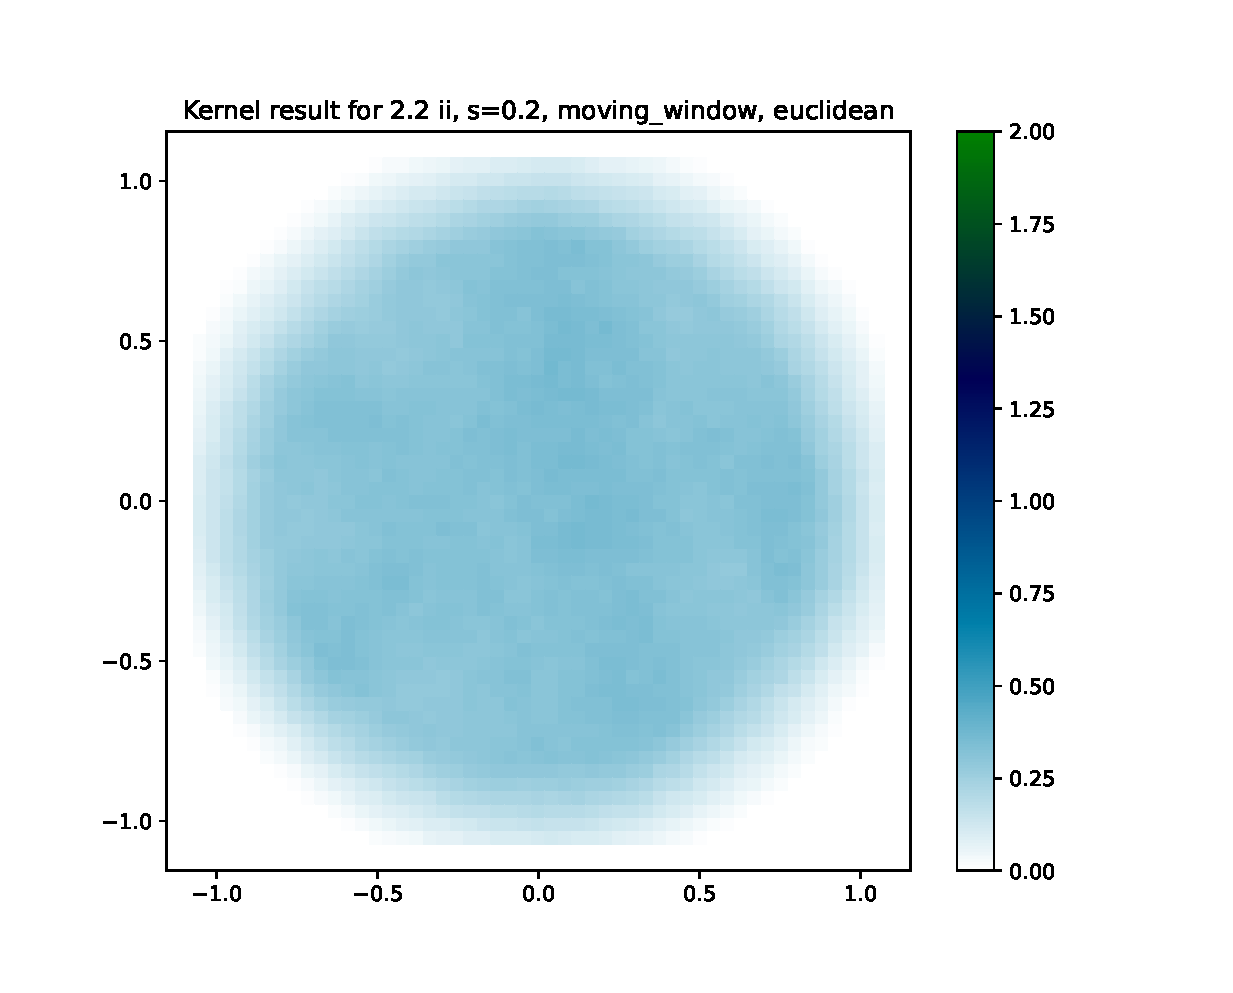
\includegraphics[height=8cm]{comparisons//Kernel_result_2-2ii_s_0-2_moving_window_euclidean.eps} \hspace*{-1.5cm}
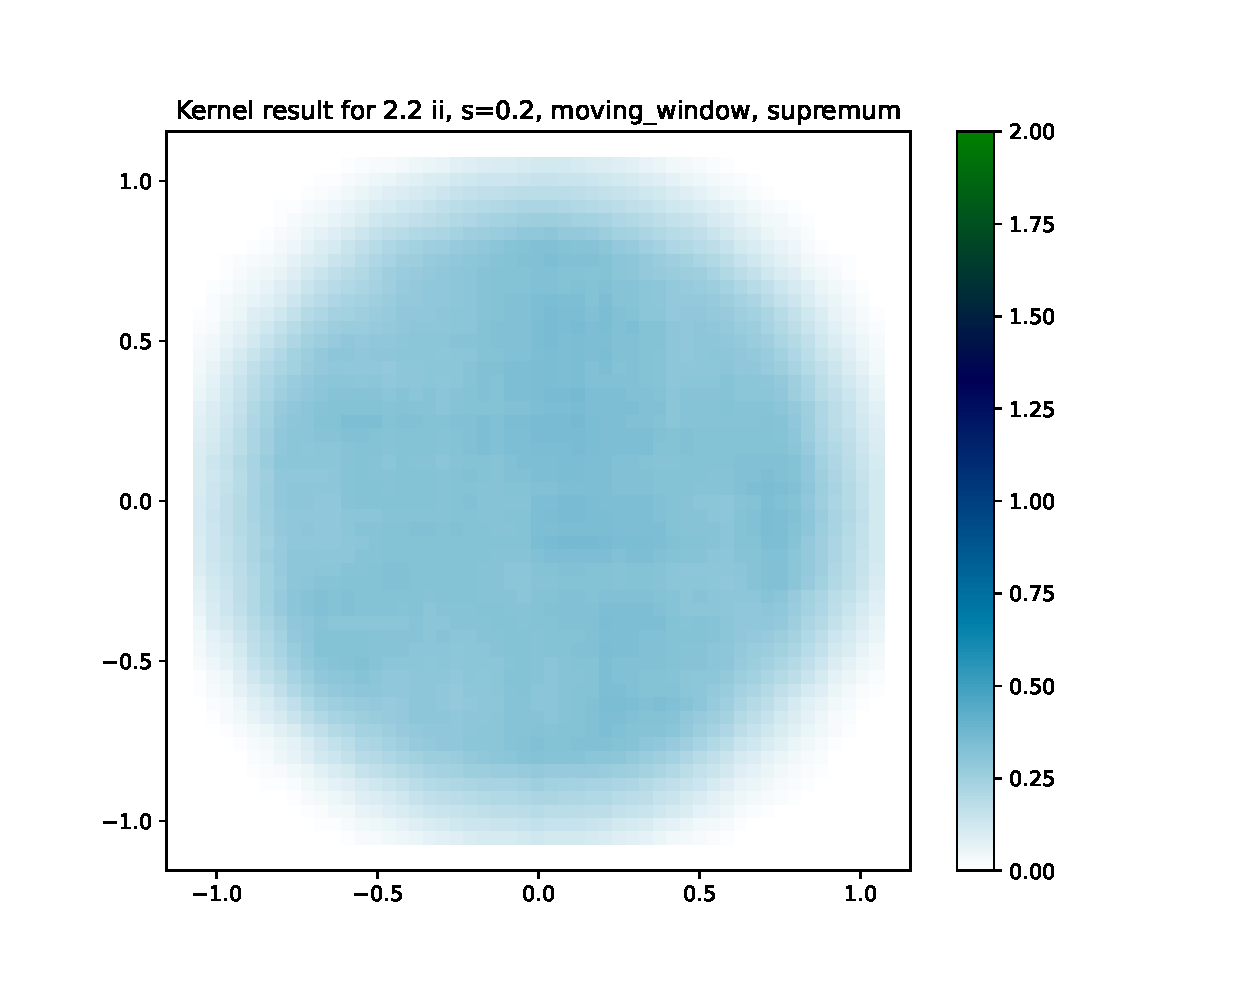
\includegraphics[height=8cm]{comparisons//Kernel_result_2-2ii_s_0-2_moving_window_supremum.eps} \\
\fi
\hspace*{-1.5cm}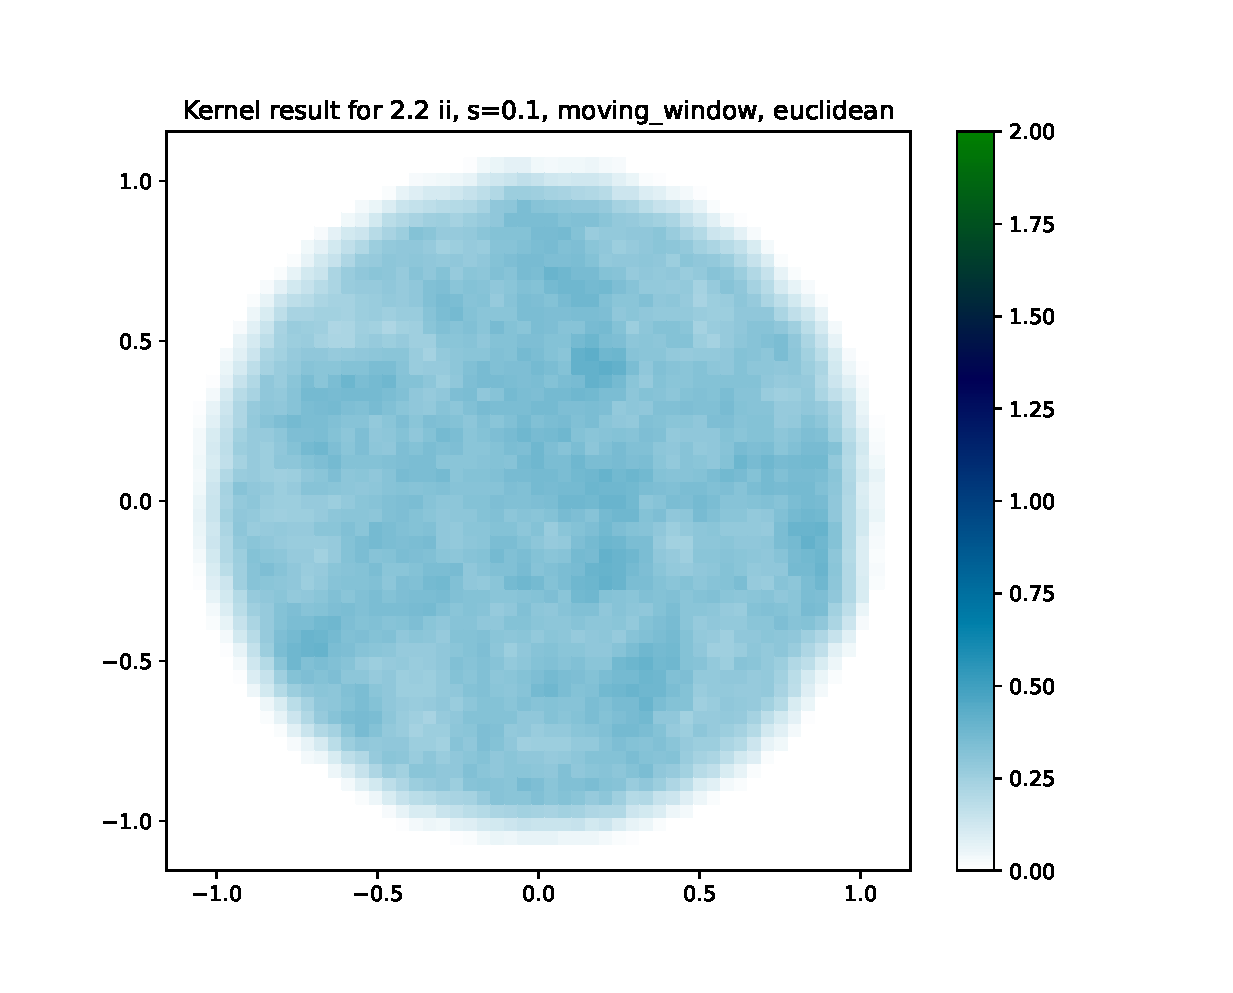
\includegraphics[height=8cm]{comparisons//Kernel_result_2-2ii_s_0-1_moving_window_euclidean.eps} \hspace*{-1.5cm}
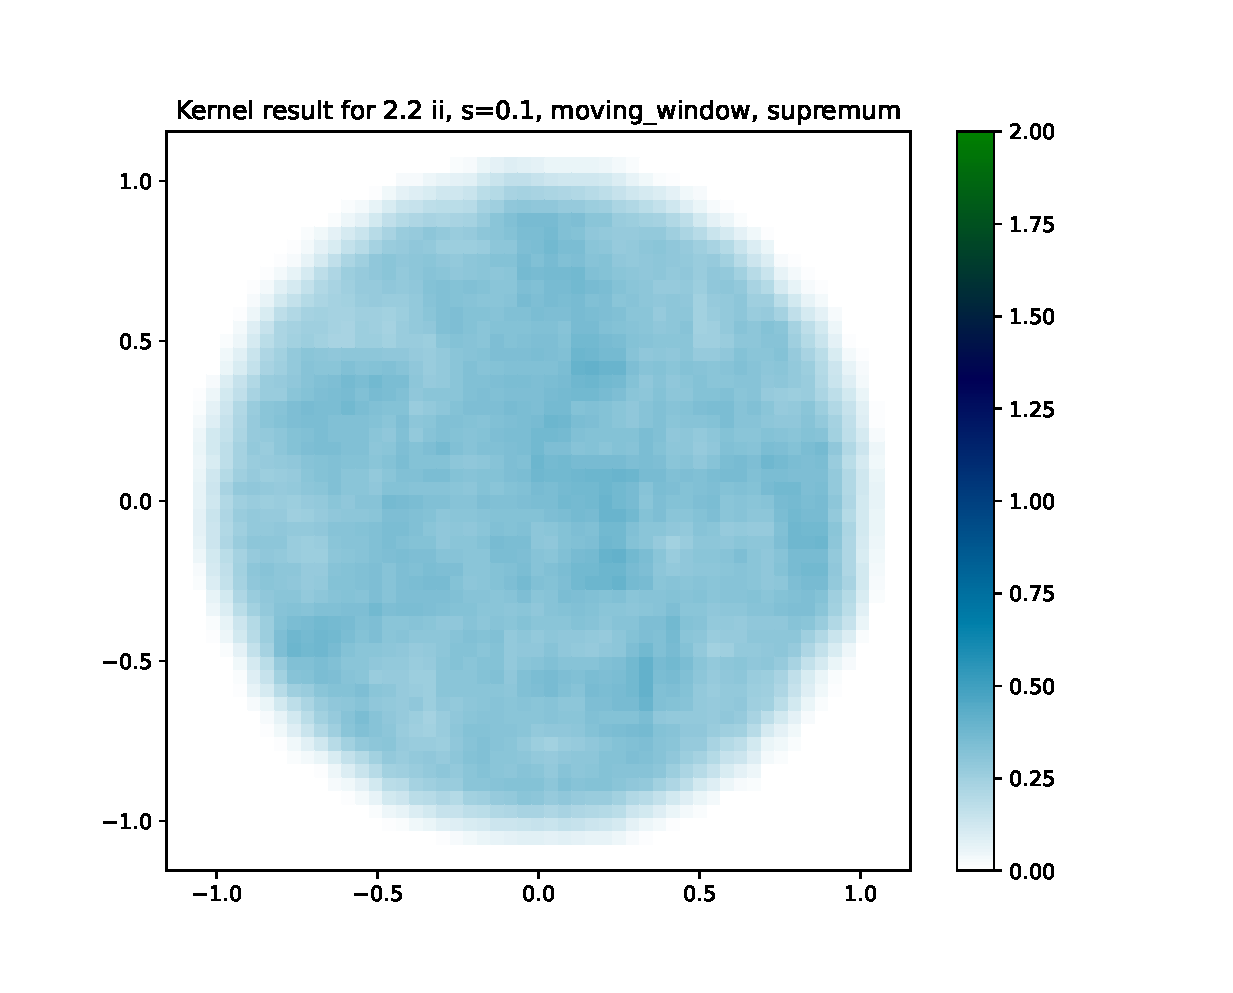
\includegraphics[height=8cm]{comparisons//Kernel_result_2-2ii_s_0-1_moving_window_supremum.eps}\\
\hspace*{-1.5cm}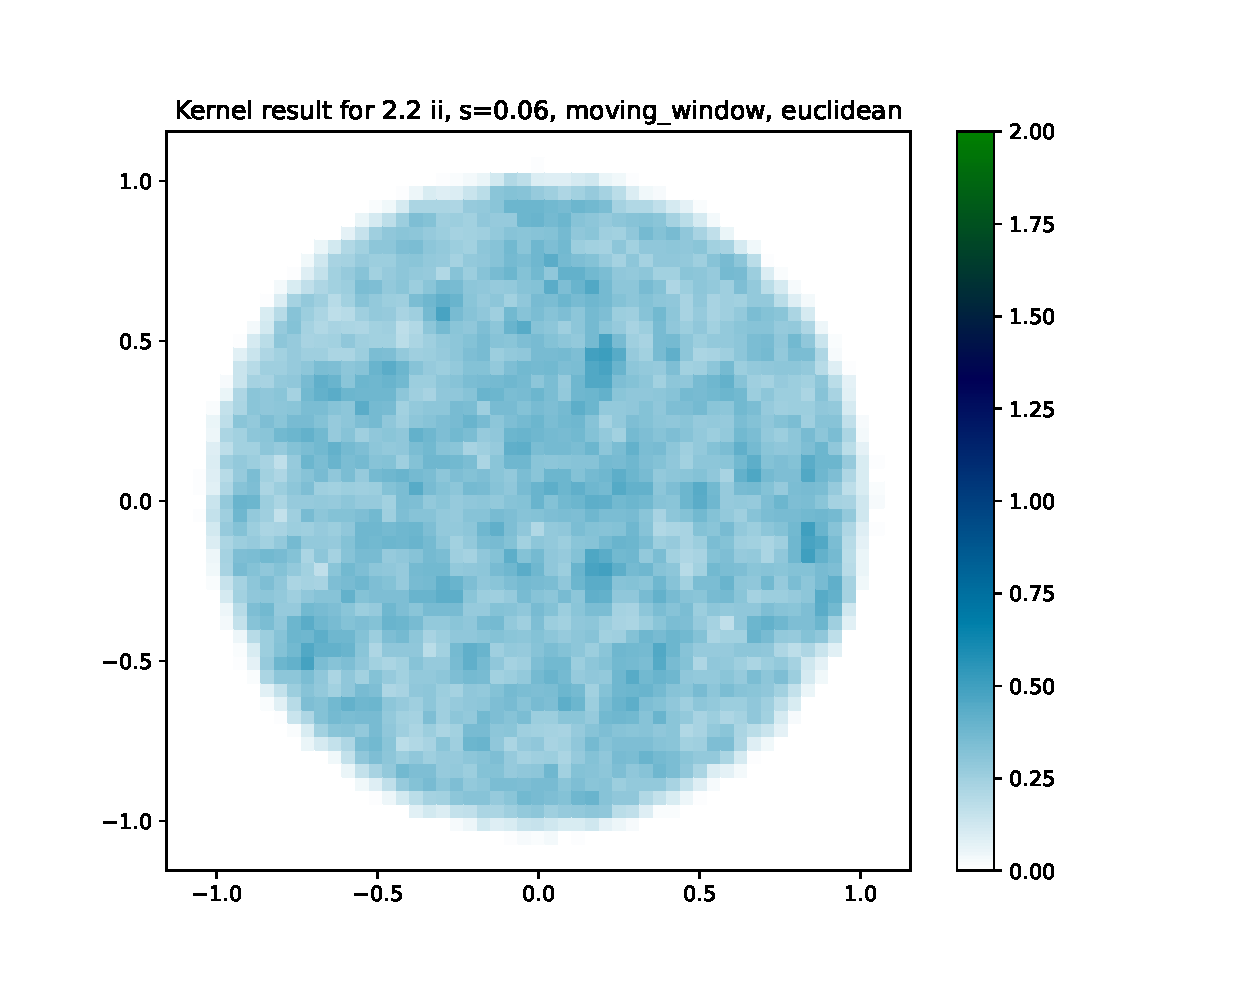
\includegraphics[height=8cm]{comparisons//Kernel_result_2-2ii_s_0-06_moving_window_euclidean.eps} \hspace*{-1.5cm}
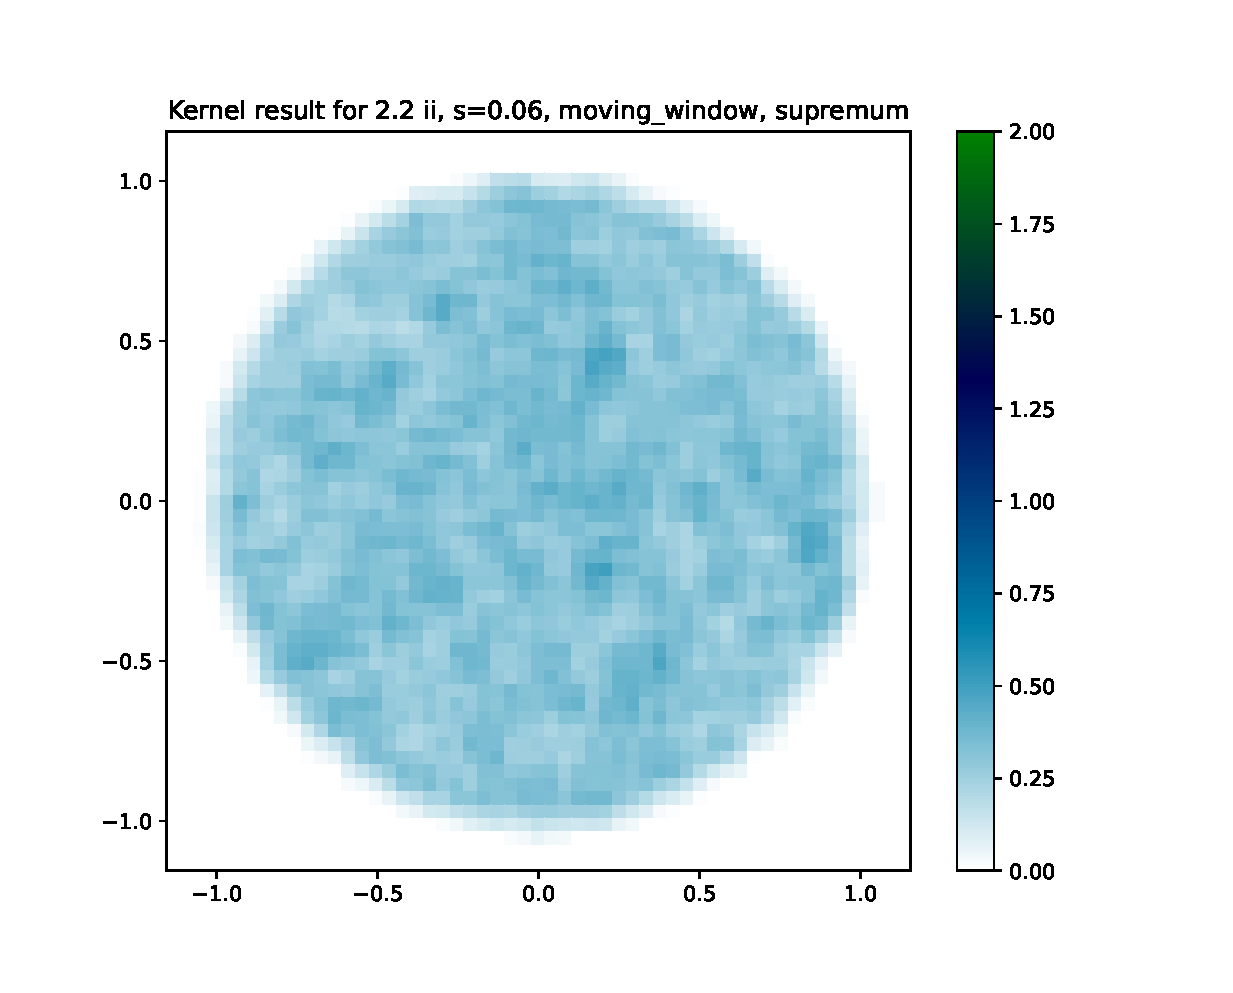
\includegraphics[height=8cm]{comparisons//Kernel_result_2-2ii_s_0-06_moving_window_supremum.eps} \\
\hspace*{-1.5cm}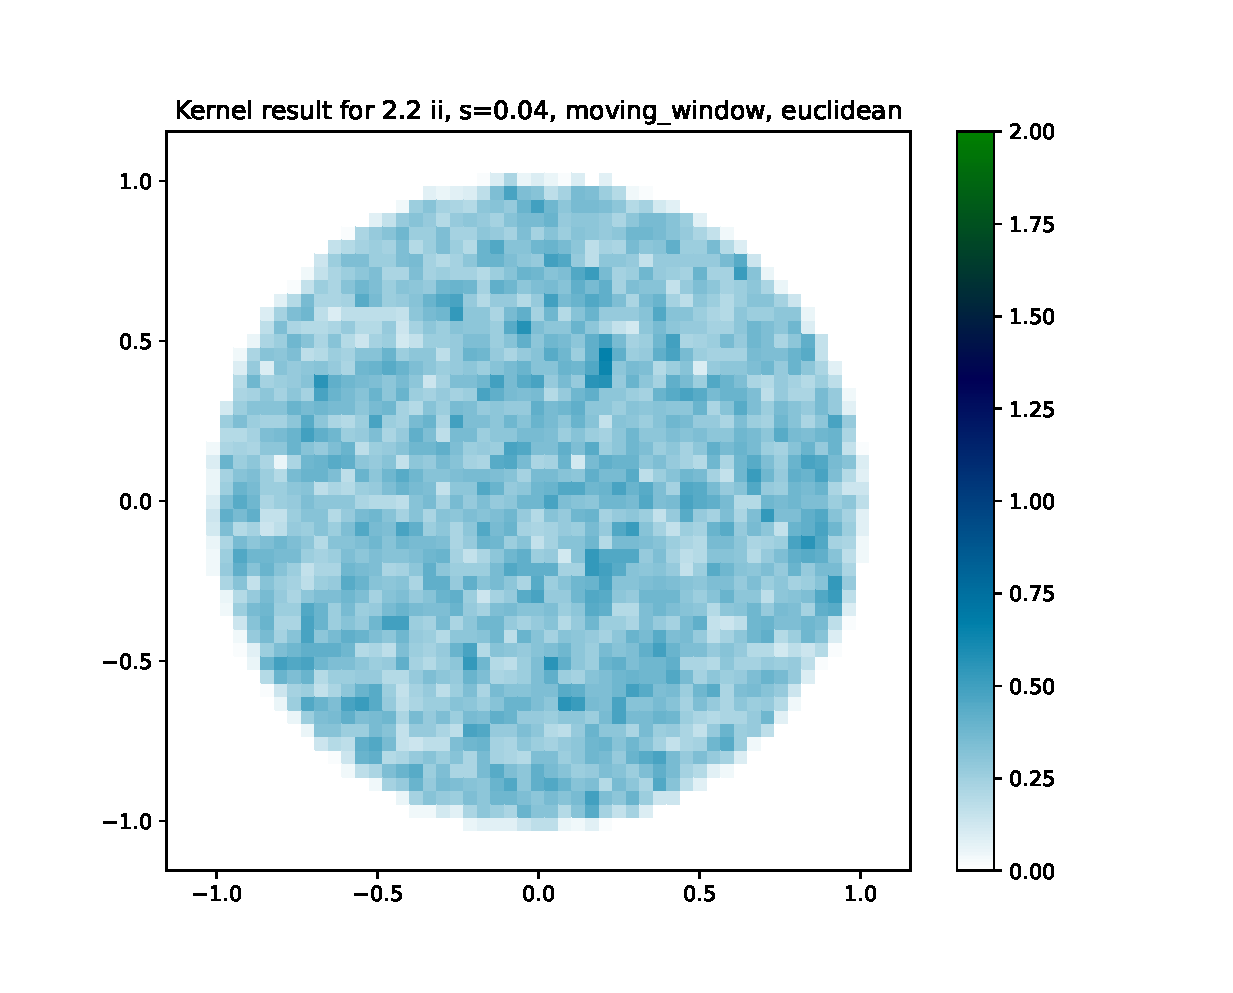
\includegraphics[height=8cm]{comparisons//Kernel_result_2-2ii_s_0-04_moving_window_euclidean.eps} \hspace*{-1.5cm}
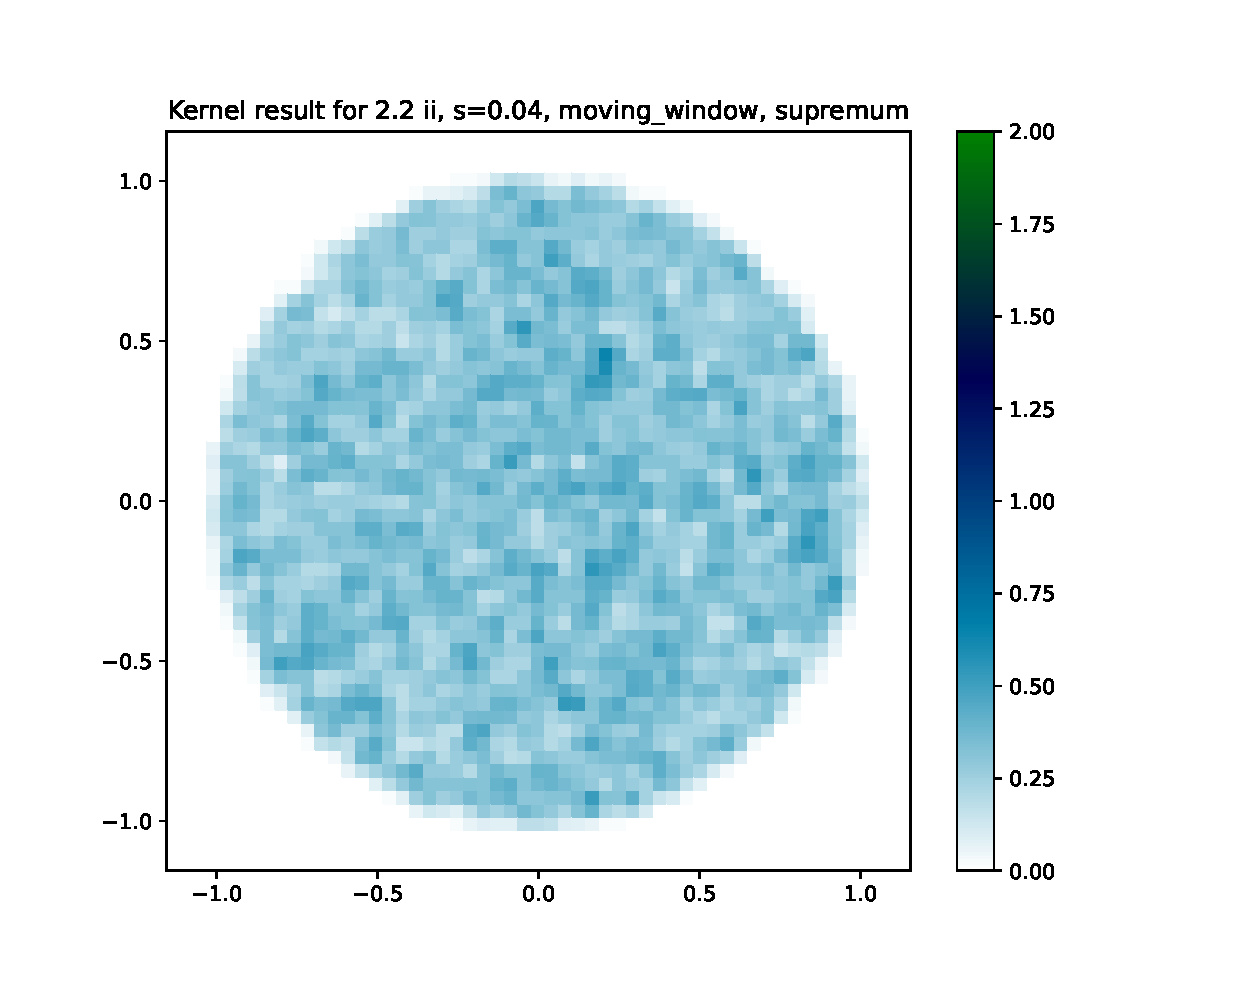
\includegraphics[height=8cm]{comparisons//Kernel_result_2-2ii_s_0-04_moving_window_supremum.eps} \\
\hspace*{-1.5cm}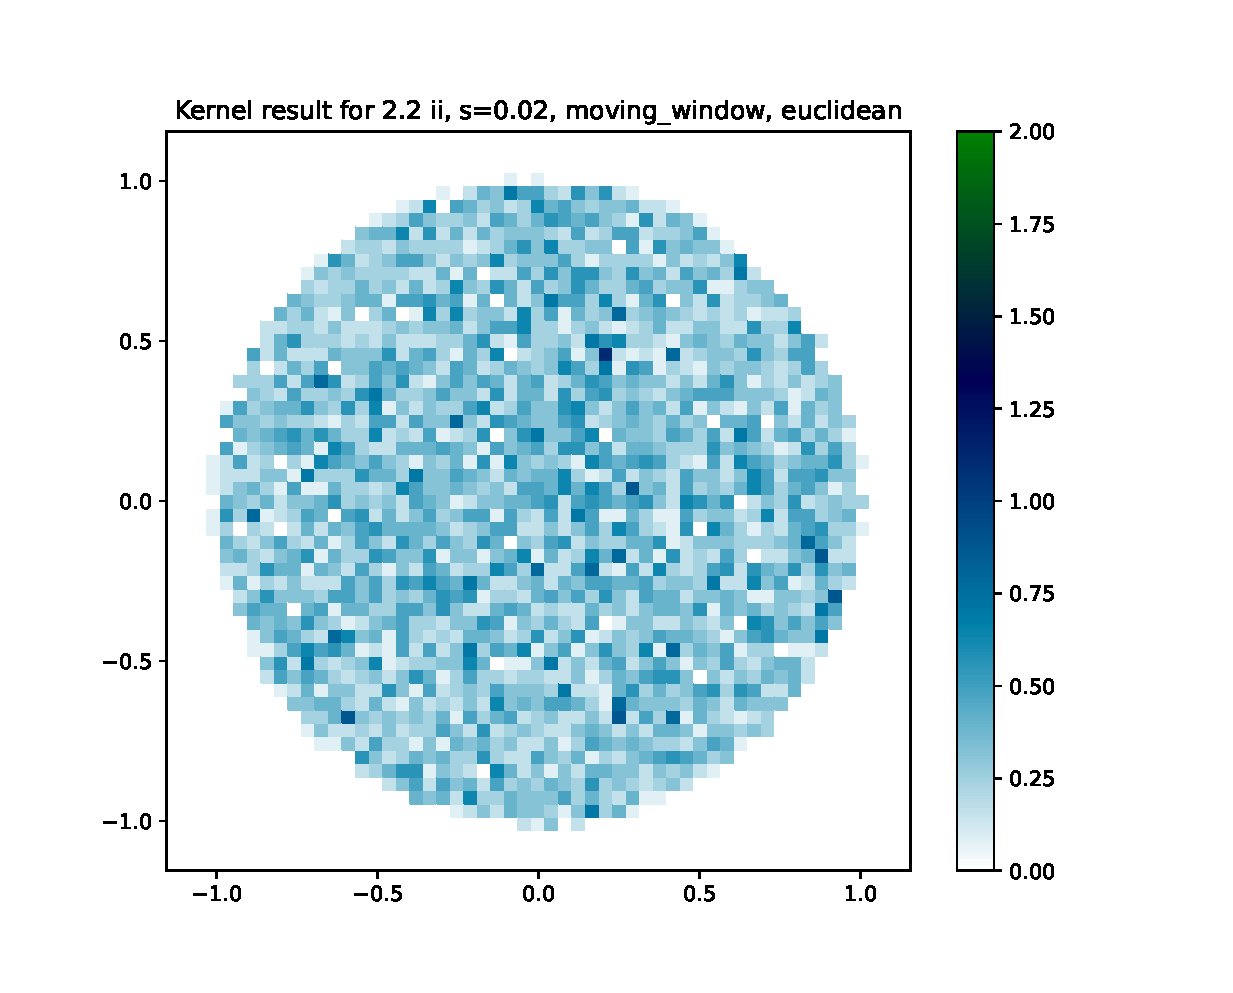
\includegraphics[height=8cm]{comparisons//Kernel_result_2-2ii_s_0-02_moving_window_euclidean.eps} \hspace*{-1.5cm}
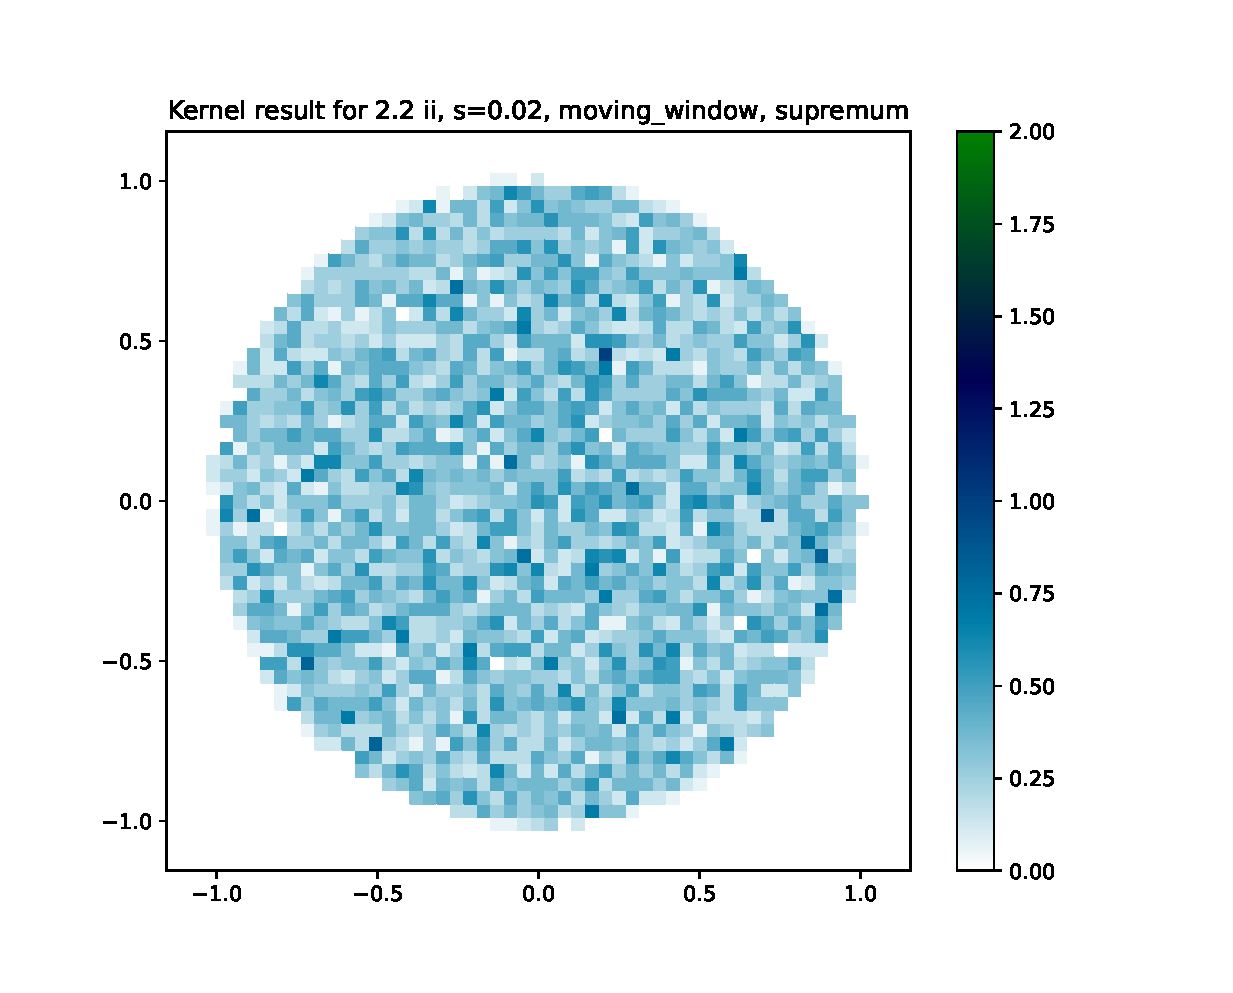
\includegraphics[height=8cm]{comparisons//Kernel_result_2-2ii_s_0-02_moving_window_supremum.eps}\\
\hspace*{-1.5cm}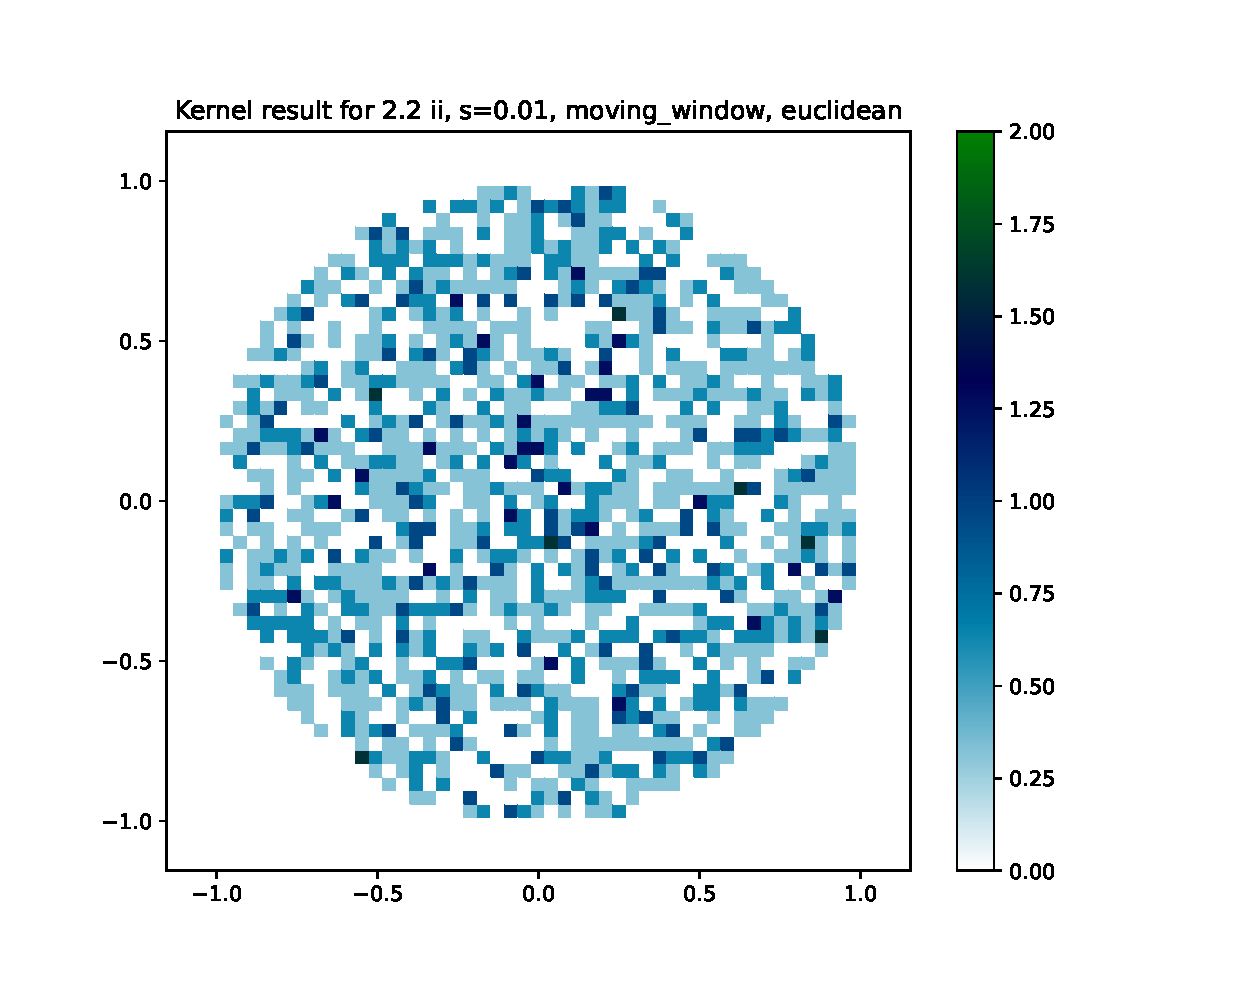
\includegraphics[height=8cm]{comparisons//Kernel_result_2-2ii_s_0-01_moving_window_euclidean.eps} \hspace*{-1.5cm}
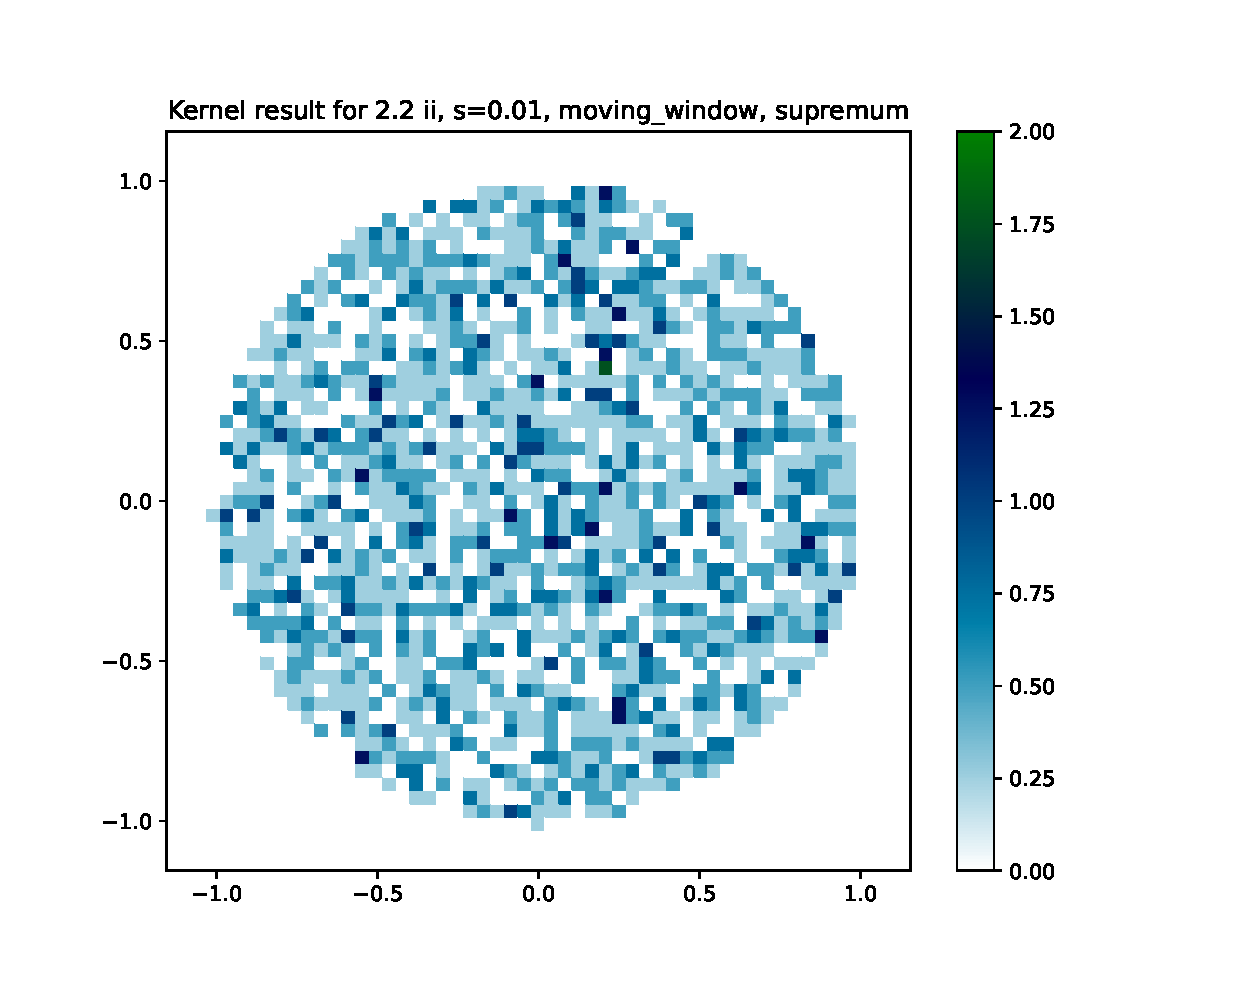
\includegraphics[height=8cm]{comparisons//Kernel_result_2-2ii_s_0-01_moving_window_supremum.eps} \vspace*{-2.5em} \\
\hspace*{-1.5cm}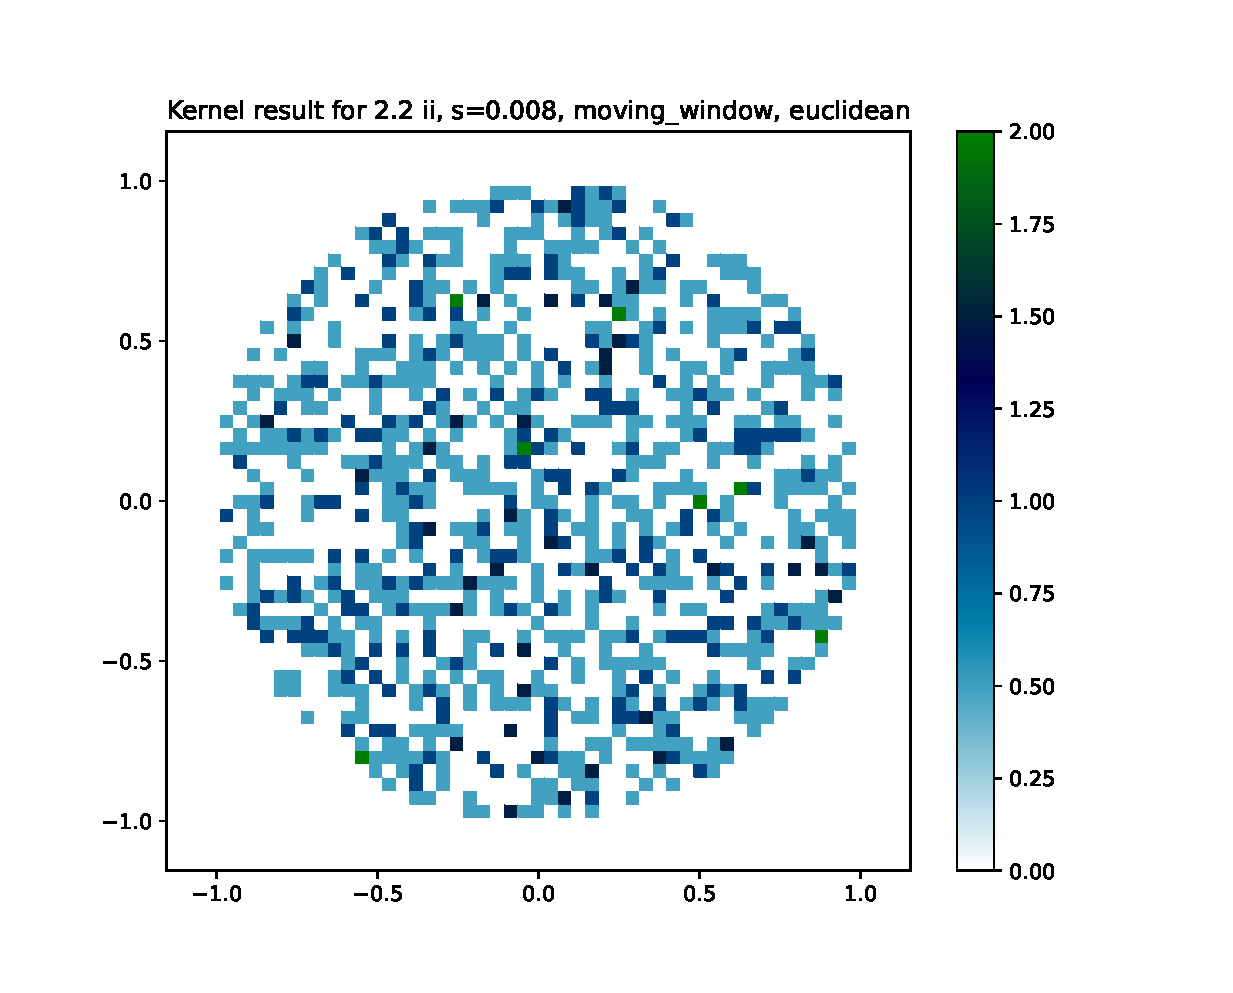
\includegraphics[height=8cm]{comparisons//Kernel_result_2-2ii_s_0-008_moving_window_euclidean.eps} \hspace*{-1.5cm}
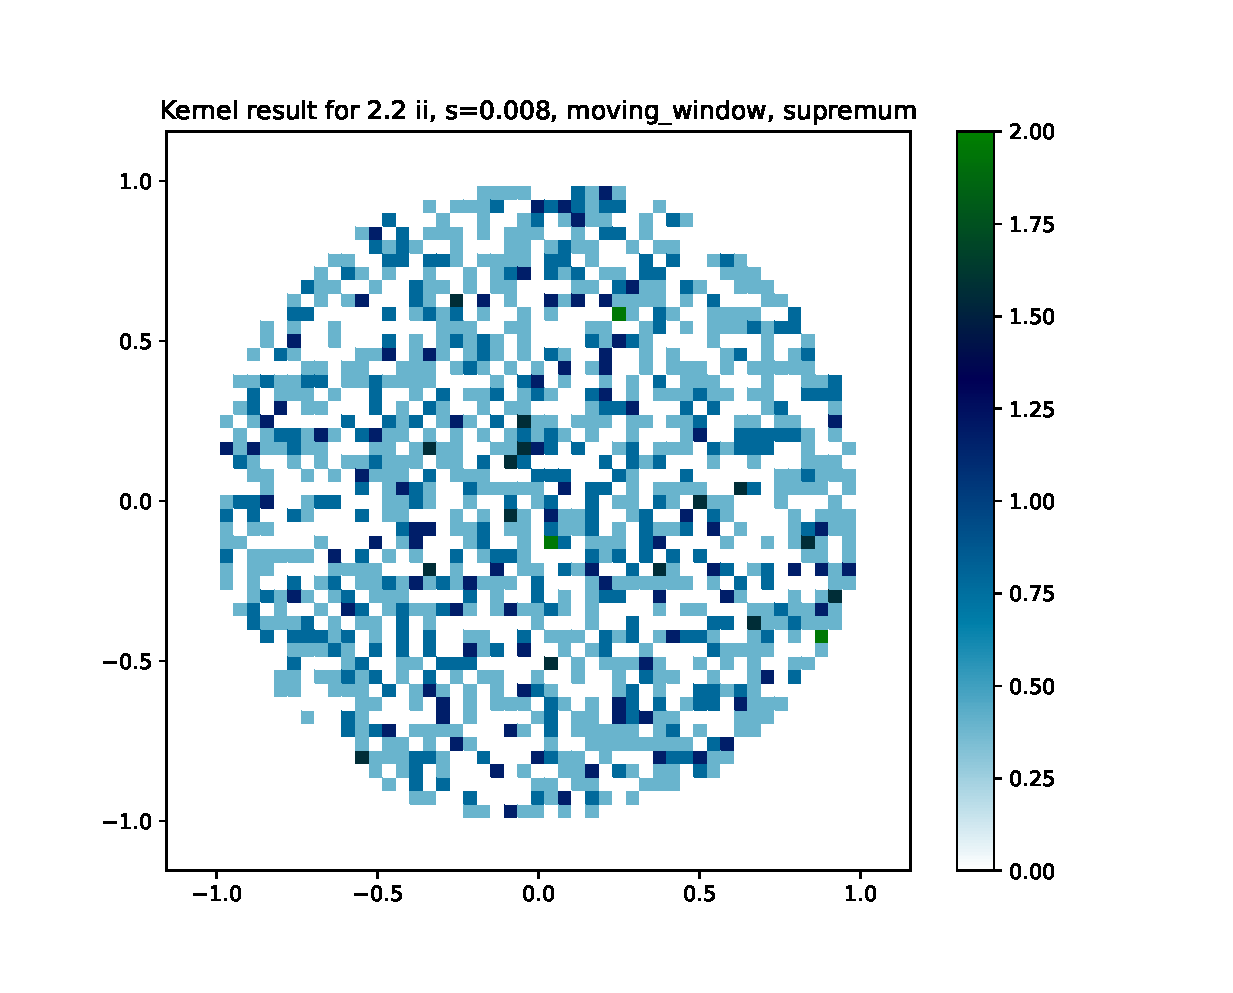
\includegraphics[height=8cm]{comparisons//Kernel_result_2-2ii_s_0-008_moving_window_supremum.eps} \vspace*{-3em} \\
\hspace*{-1.5cm}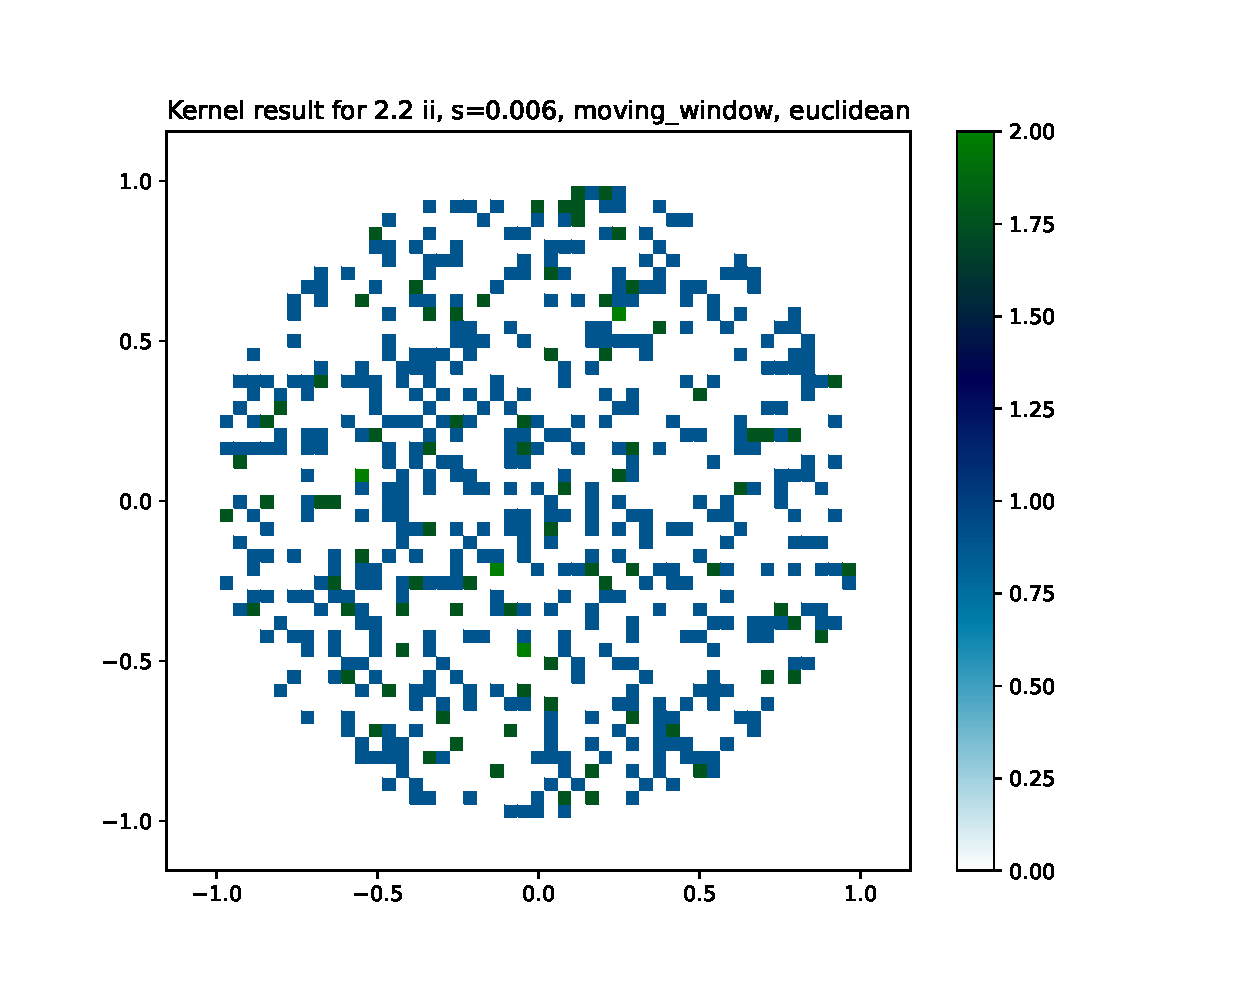
\includegraphics[height=8cm]{comparisons//Kernel_result_2-2ii_s_0-006_moving_window_euclidean.eps} \hspace*{-1.5cm}
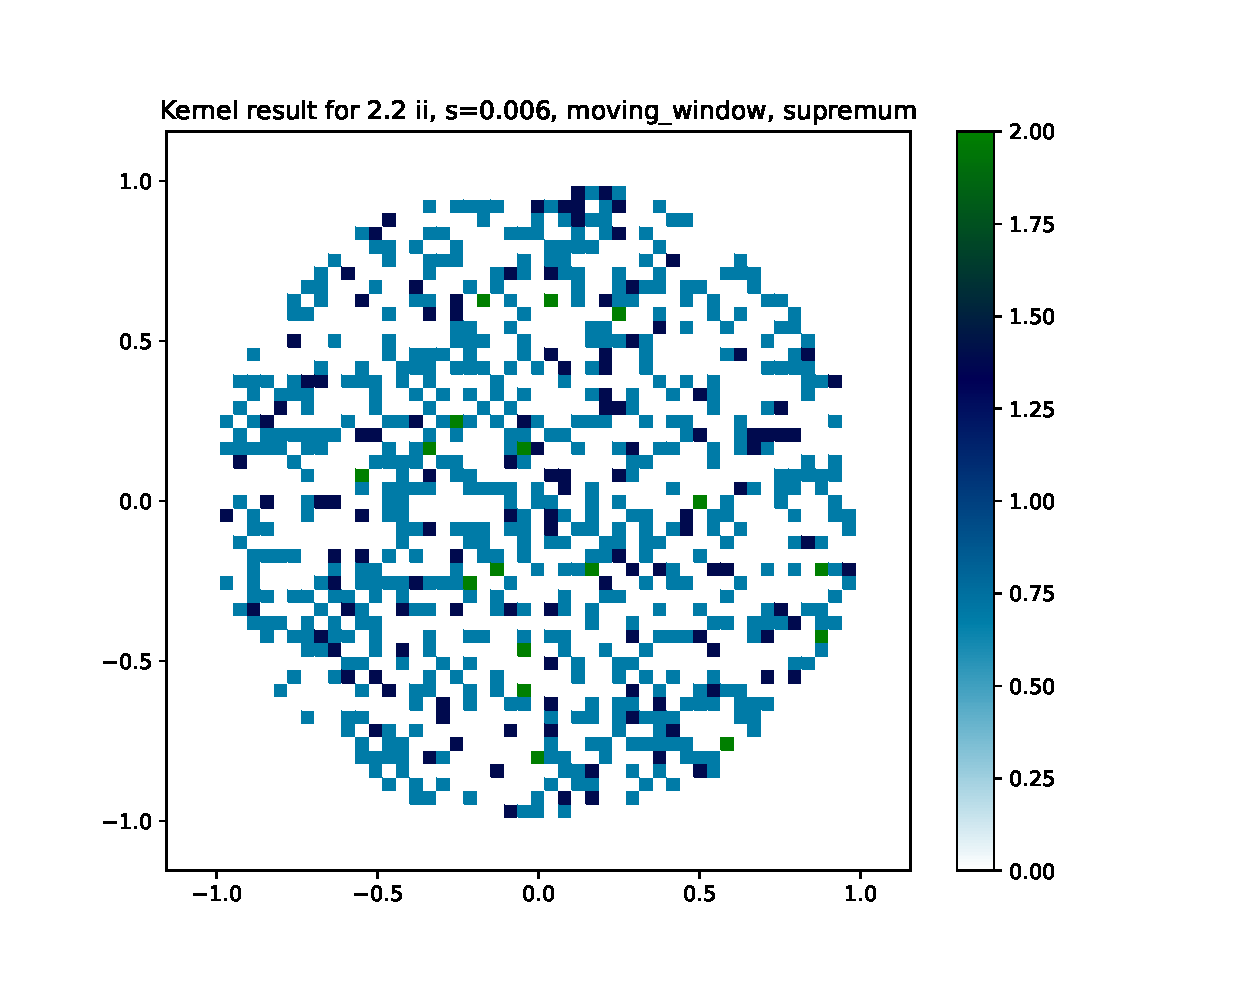
\includegraphics[height=8cm]{comparisons//Kernel_result_2-2ii_s_0-006_moving_window_supremum.eps} \vspace*{-2em} \\
What we see is that the choice of norm is seemingly less influencial, and that with decreasing $s$, the accuracy of the estimation seems to firstly grow but then decrease. \\
\noindent Secondly, we compare the results of Moving Window kernel with Gaussian kernel under Euclidean norm for different $s$: \\
\iffalse
\hspace*{-1.5cm}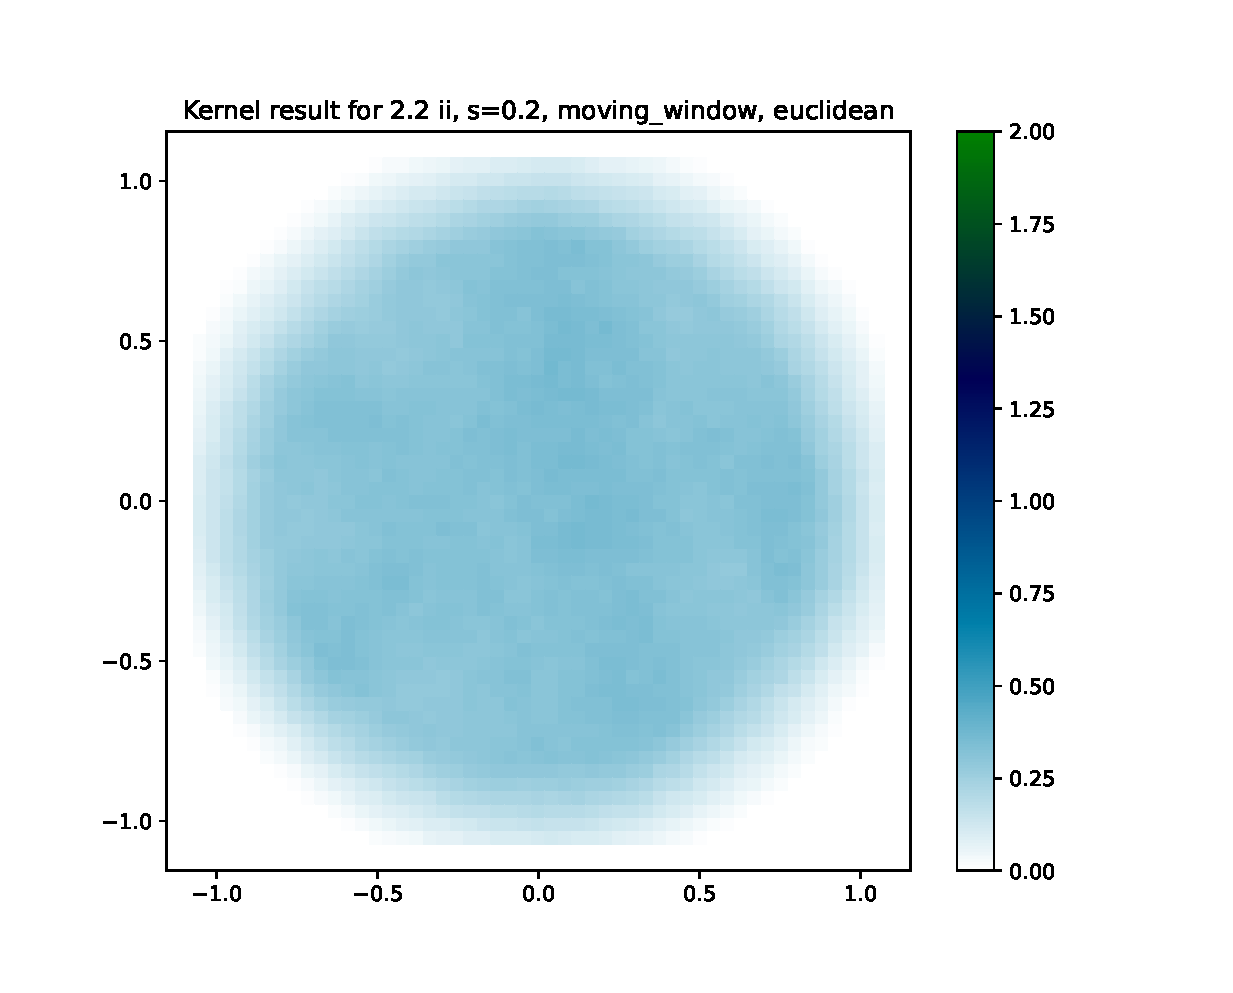
\includegraphics[height=8cm]{comparisons//Kernel_result_2-2ii_s_0-2_moving_window_euclidean.eps} \hspace*{-1.5cm}
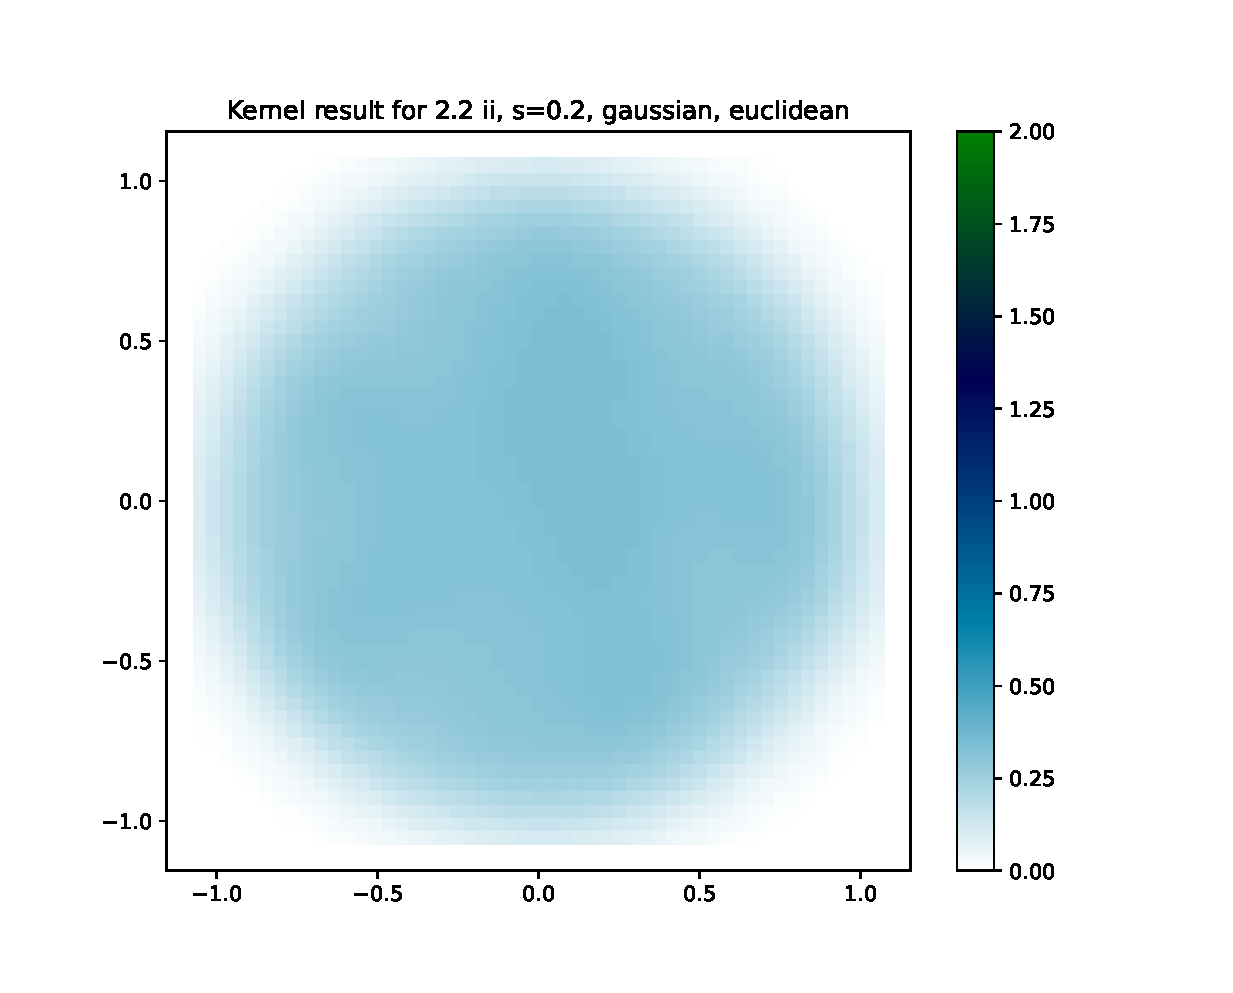
\includegraphics[height=8cm]{comparisons//Kernel_result_2-2ii_s_0-2_gaussian_euclidean.eps} \vspace*{-3em} \\
\fi
\hspace*{-1.5cm}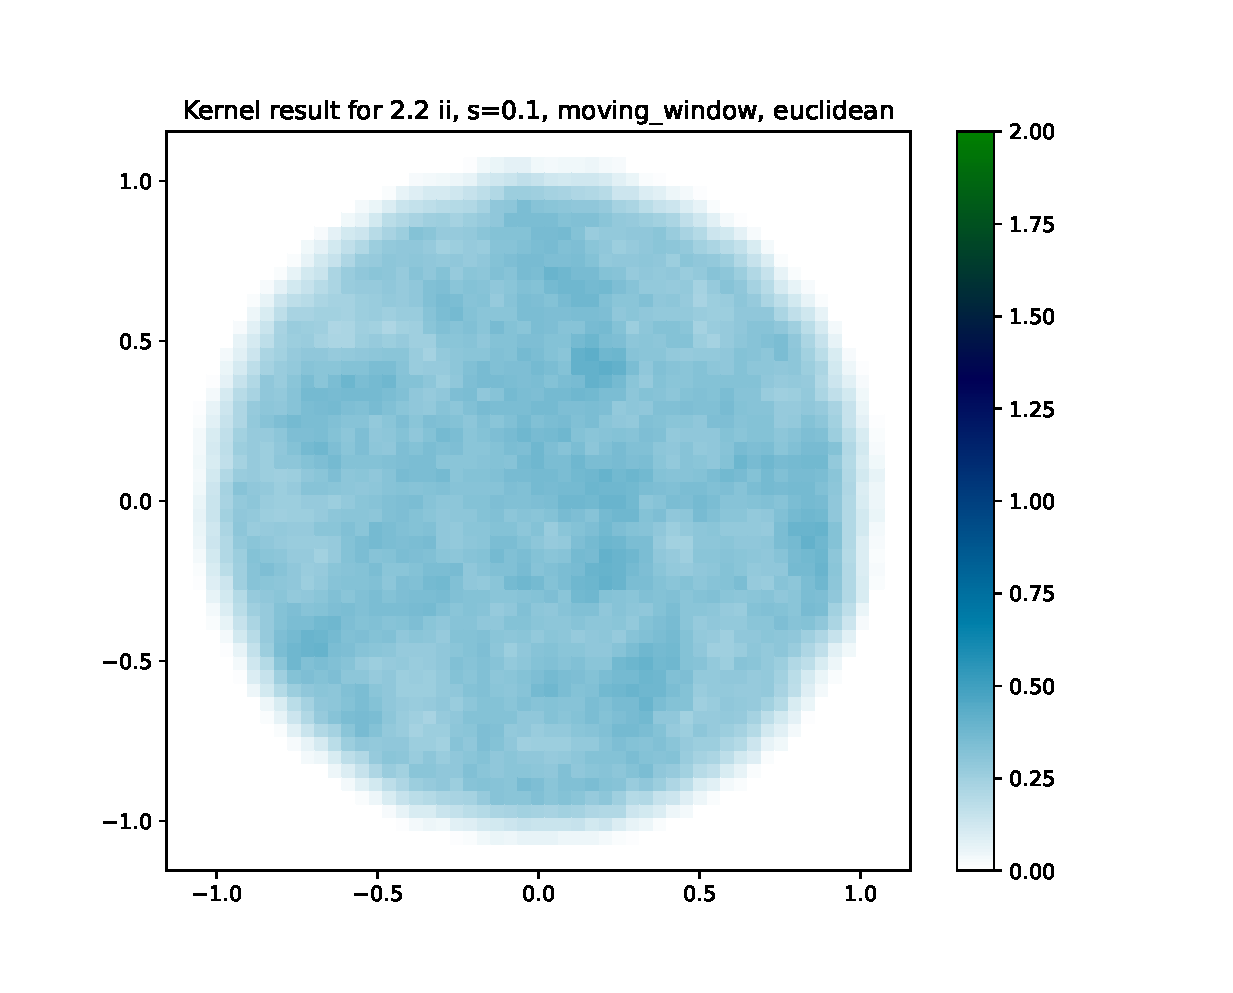
\includegraphics[height=8cm]{comparisons//Kernel_result_2-2ii_s_0-1_moving_window_euclidean.eps} \hspace*{-1.5cm}
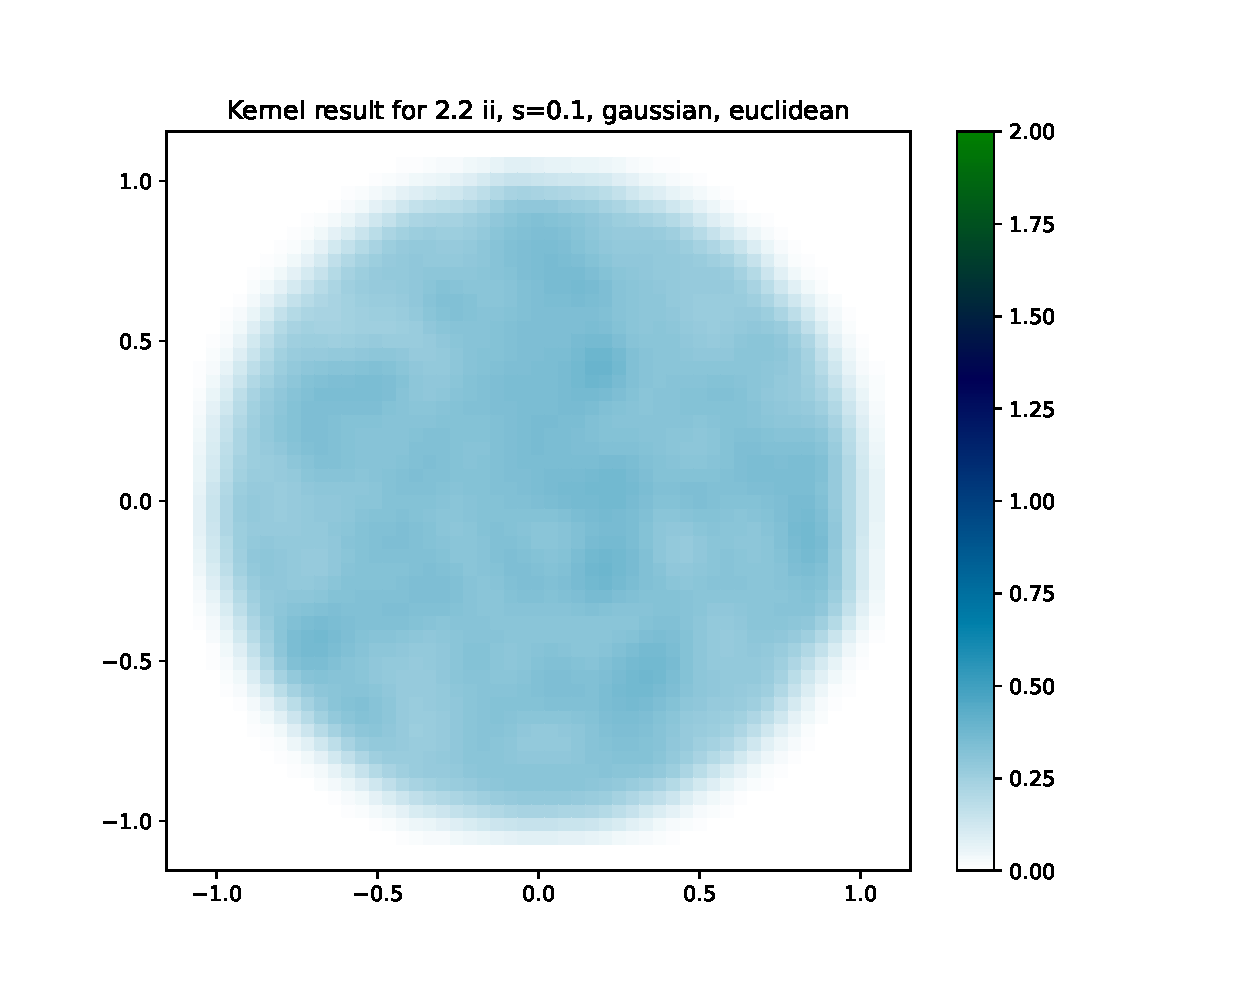
\includegraphics[height=8cm]{comparisons//Kernel_result_2-2ii_s_0-1_gaussian_euclidean.eps} \vspace*{-3em}  \\
\hspace*{-1.5cm}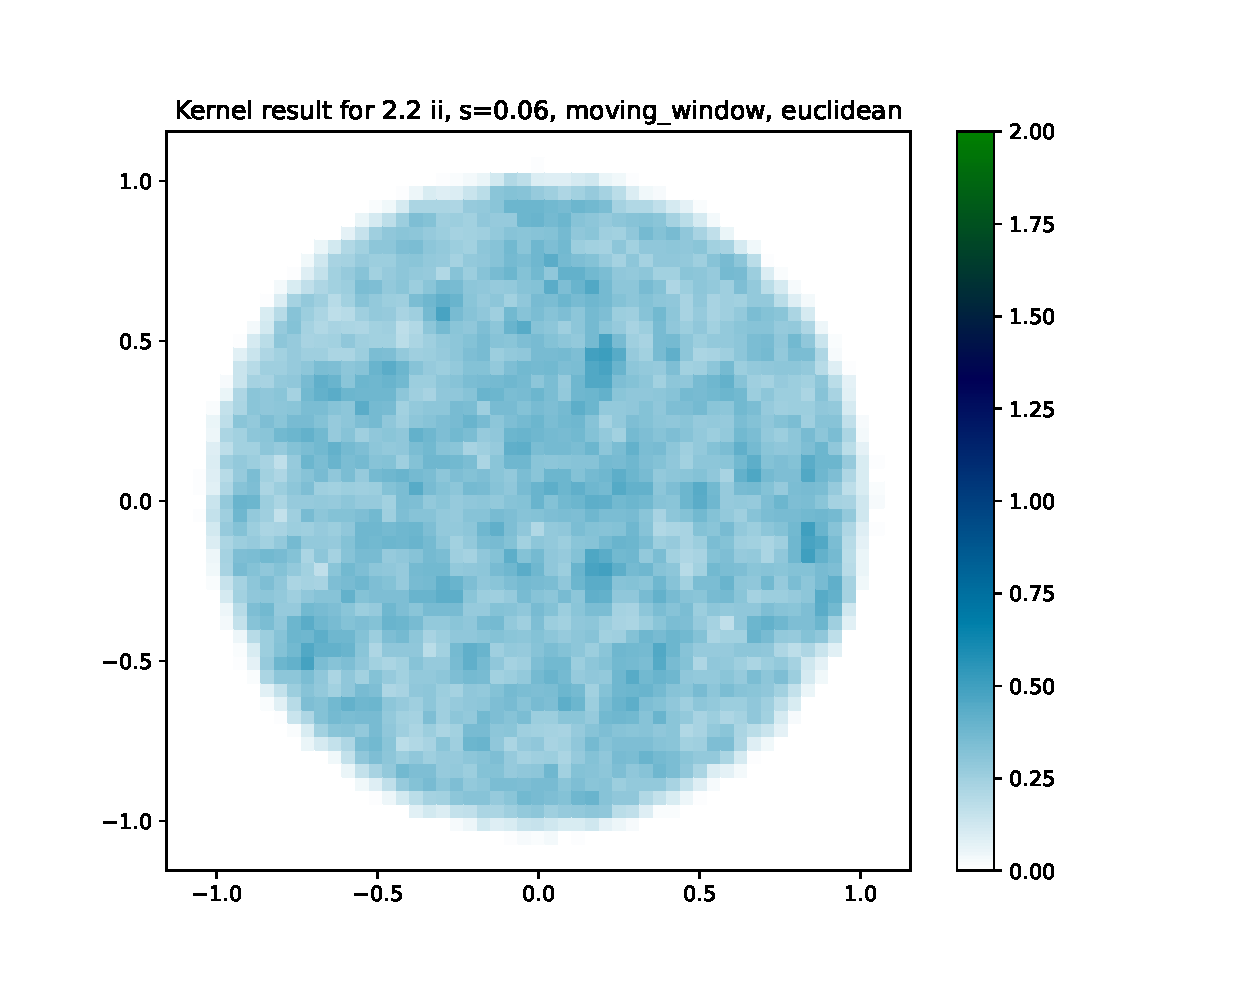
\includegraphics[height=8cm]{comparisons//Kernel_result_2-2ii_s_0-06_moving_window_euclidean.eps} \hspace*{-1.5cm}
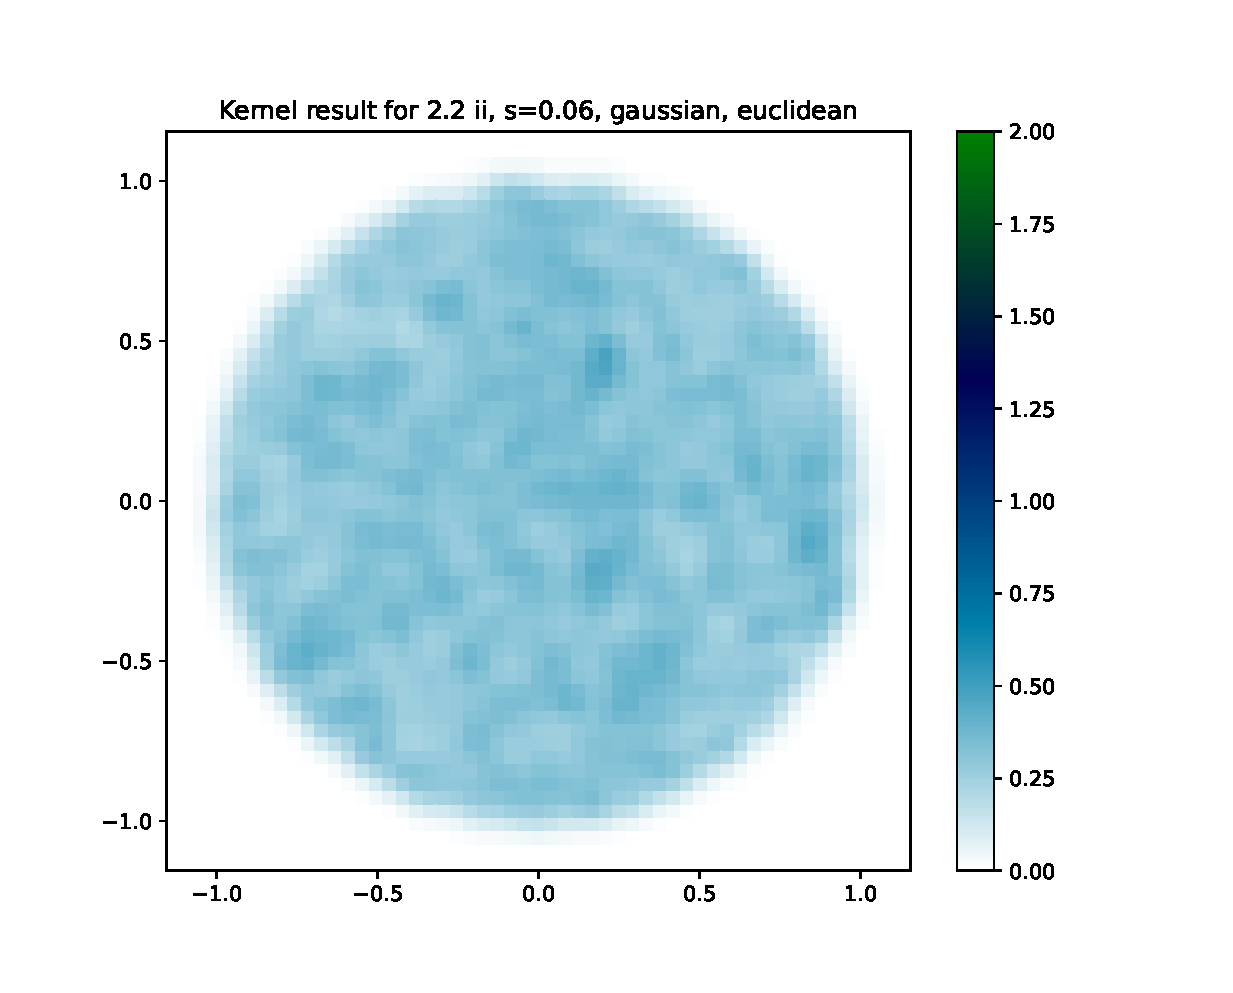
\includegraphics[height=8cm]{comparisons//Kernel_result_2-2ii_s_0-06_gaussian_euclidean.eps}  \\
\hspace*{-1.5cm}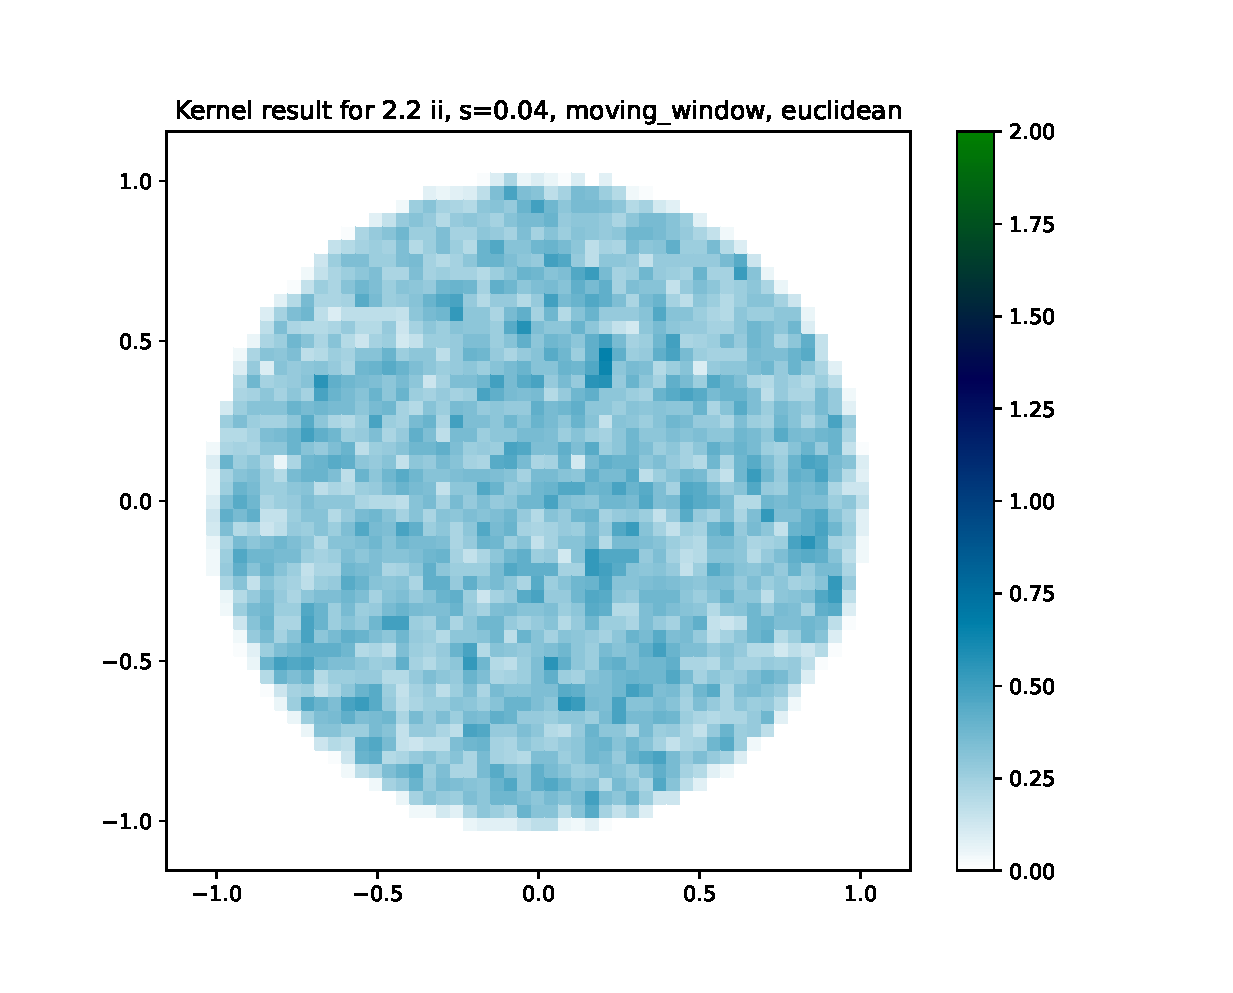
\includegraphics[height=8cm]{comparisons//Kernel_result_2-2ii_s_0-04_moving_window_euclidean.eps} \hspace*{-1.5cm}
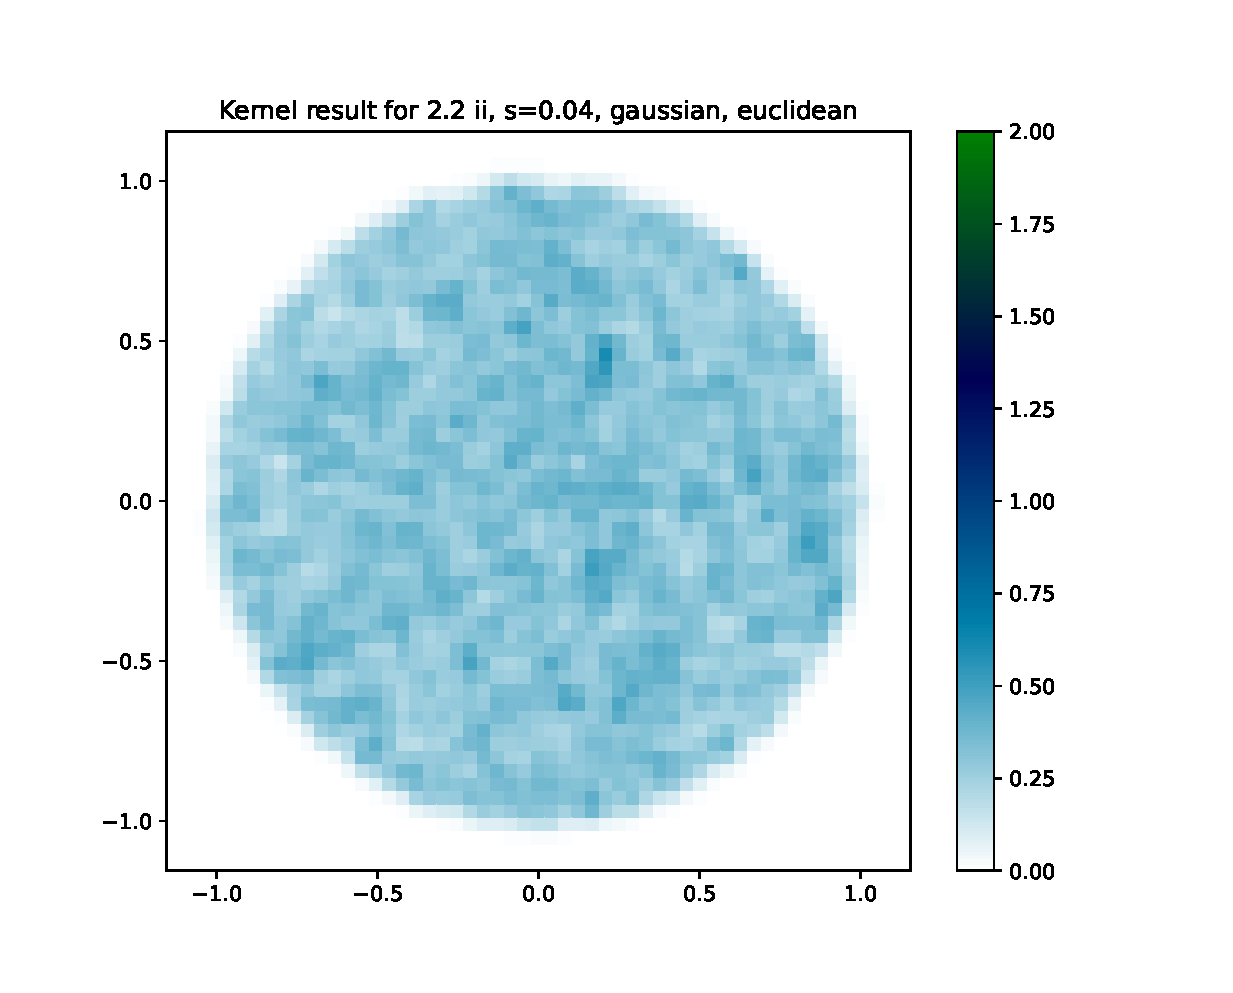
\includegraphics[height=8cm]{comparisons//Kernel_result_2-2ii_s_0-04_gaussian_euclidean.eps}  \\
\hspace*{-1.5cm}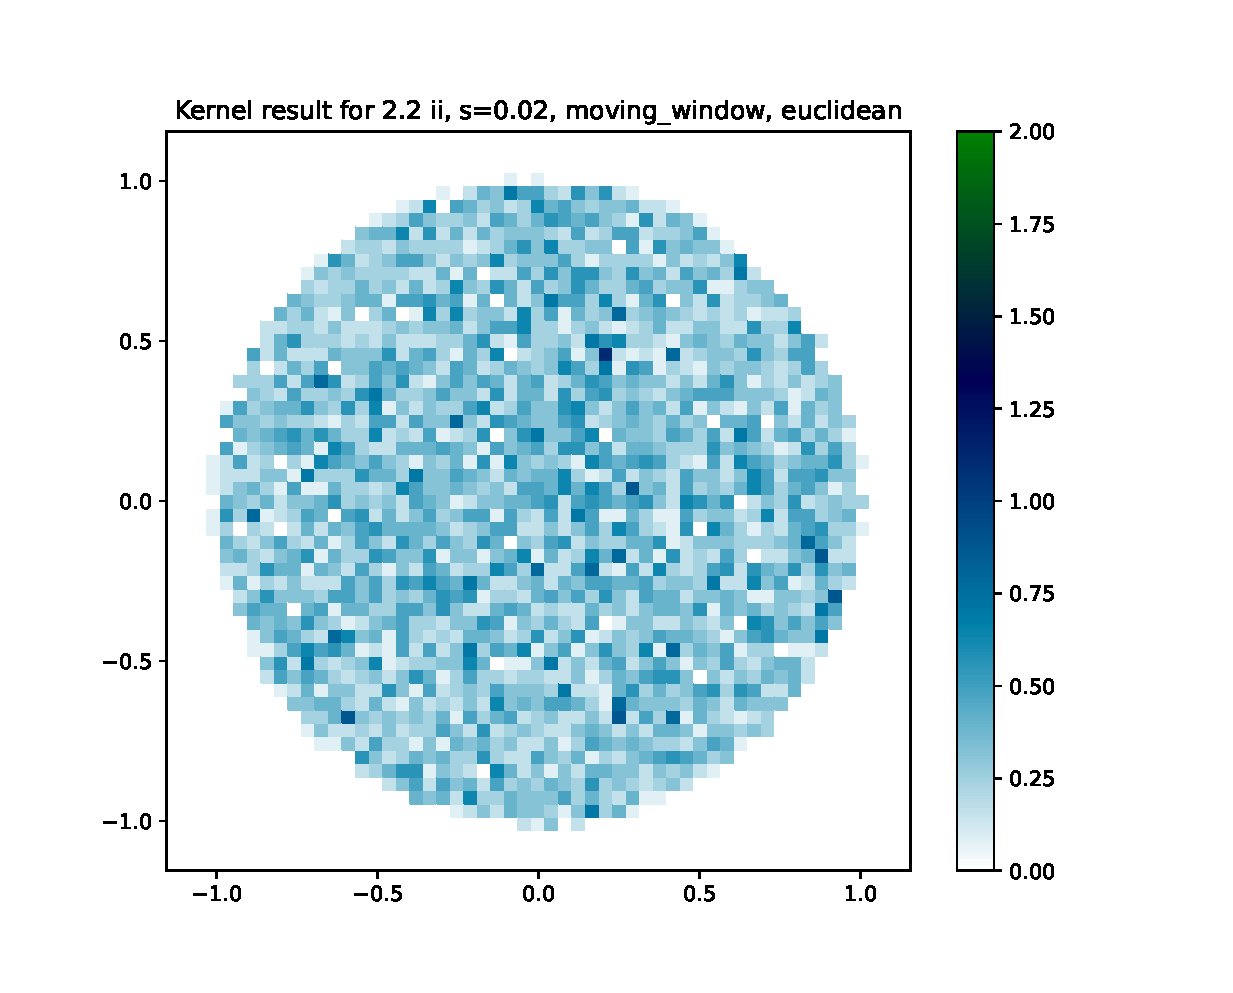
\includegraphics[height=8cm]{comparisons//Kernel_result_2-2ii_s_0-02_moving_window_euclidean.eps} \hspace*{-1.5cm}
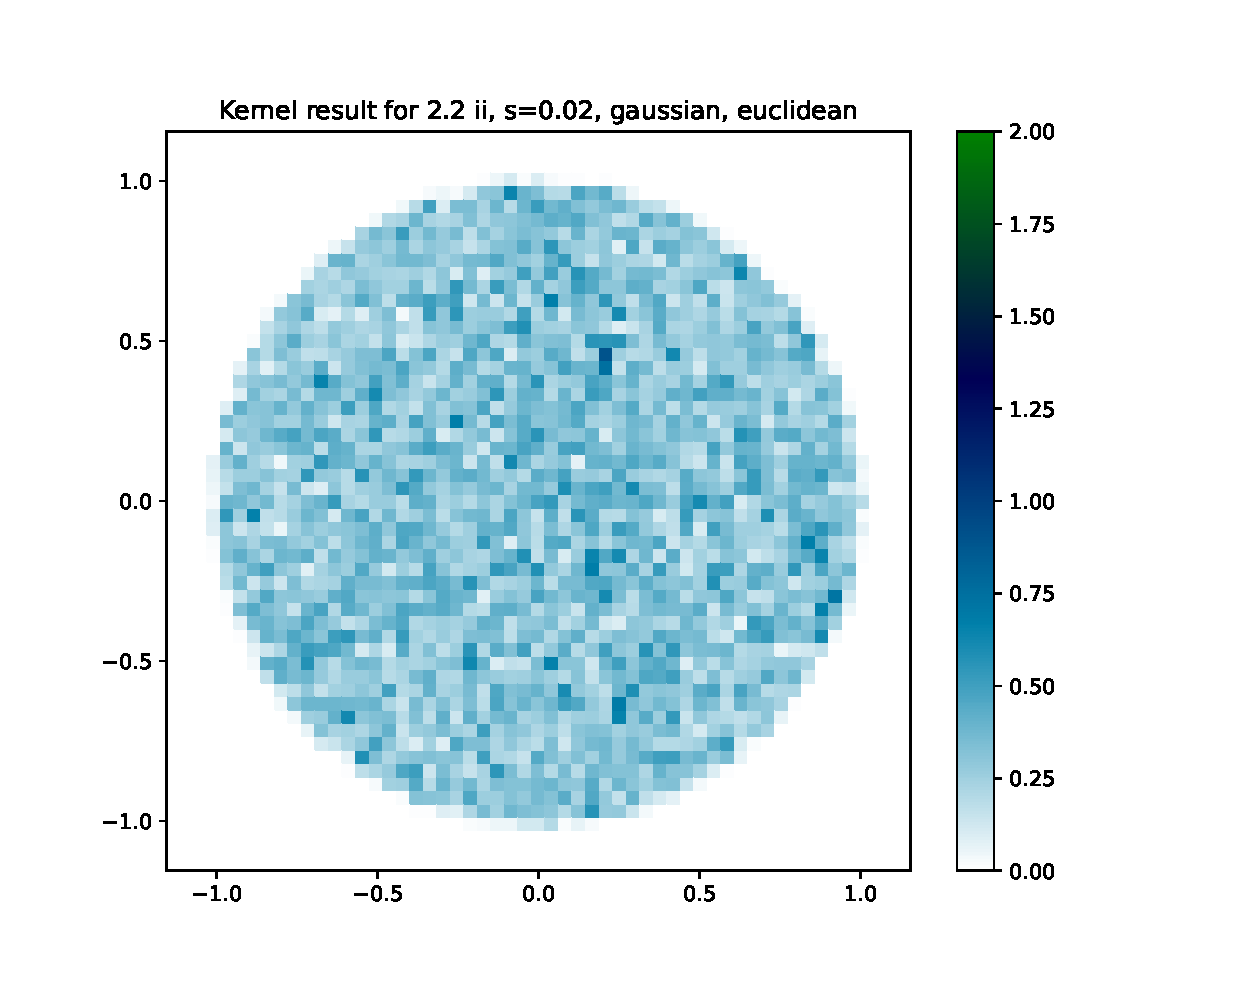
\includegraphics[height=8cm]{comparisons//Kernel_result_2-2ii_s_0-02_gaussian_euclidean.eps}  \\
\hspace*{-1.5cm}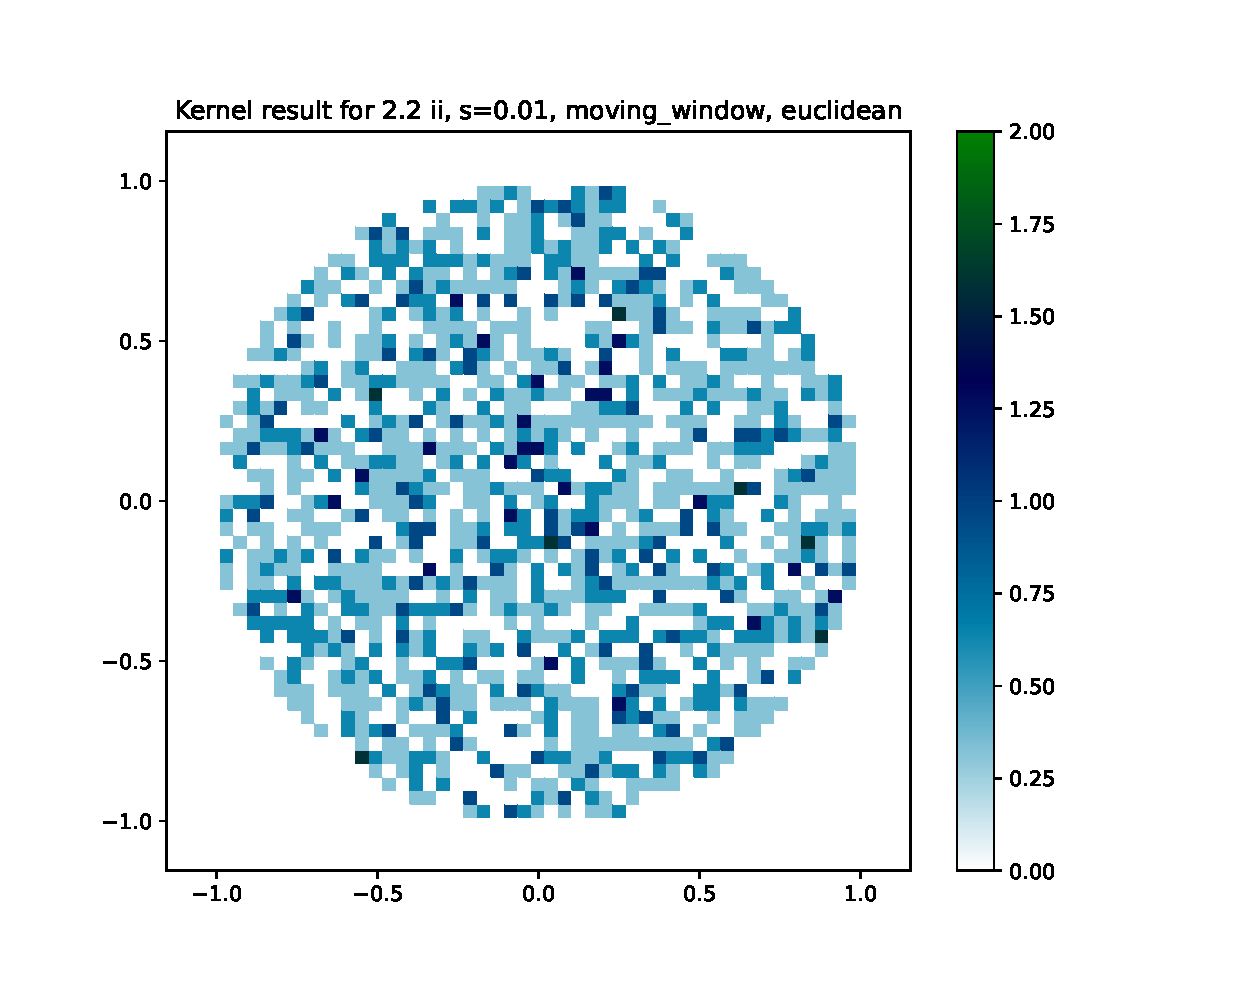
\includegraphics[height=8cm]{comparisons//Kernel_result_2-2ii_s_0-01_moving_window_euclidean.eps} \hspace*{-1.5cm}
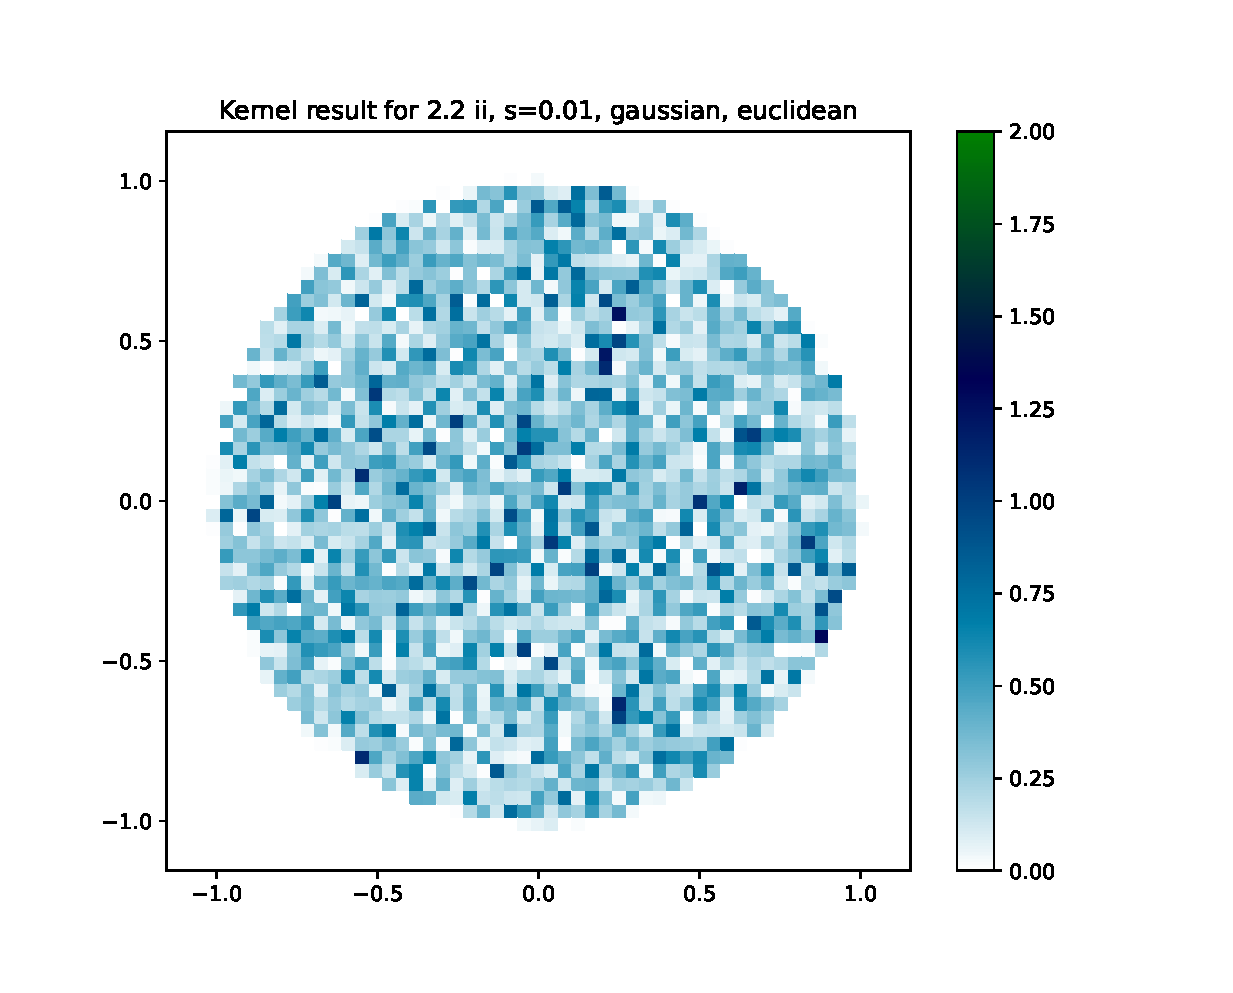
\includegraphics[height=8cm]{comparisons//Kernel_result_2-2ii_s_0-01_gaussian_euclidean.eps}  \\
\hspace*{-1.5cm}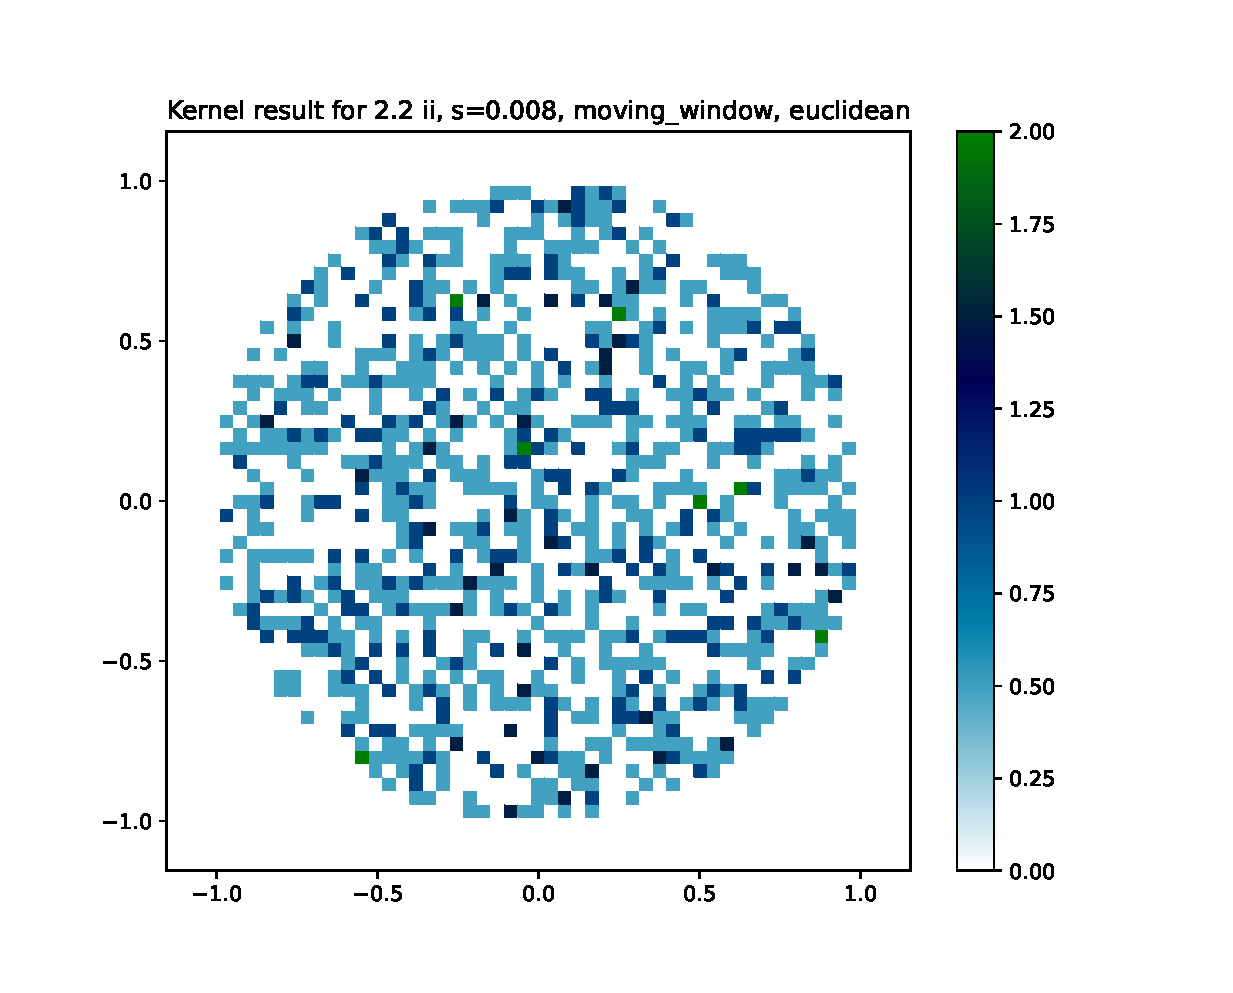
\includegraphics[height=8cm]{comparisons//Kernel_result_2-2ii_s_0-008_moving_window_euclidean.eps} \hspace*{-1.5cm}
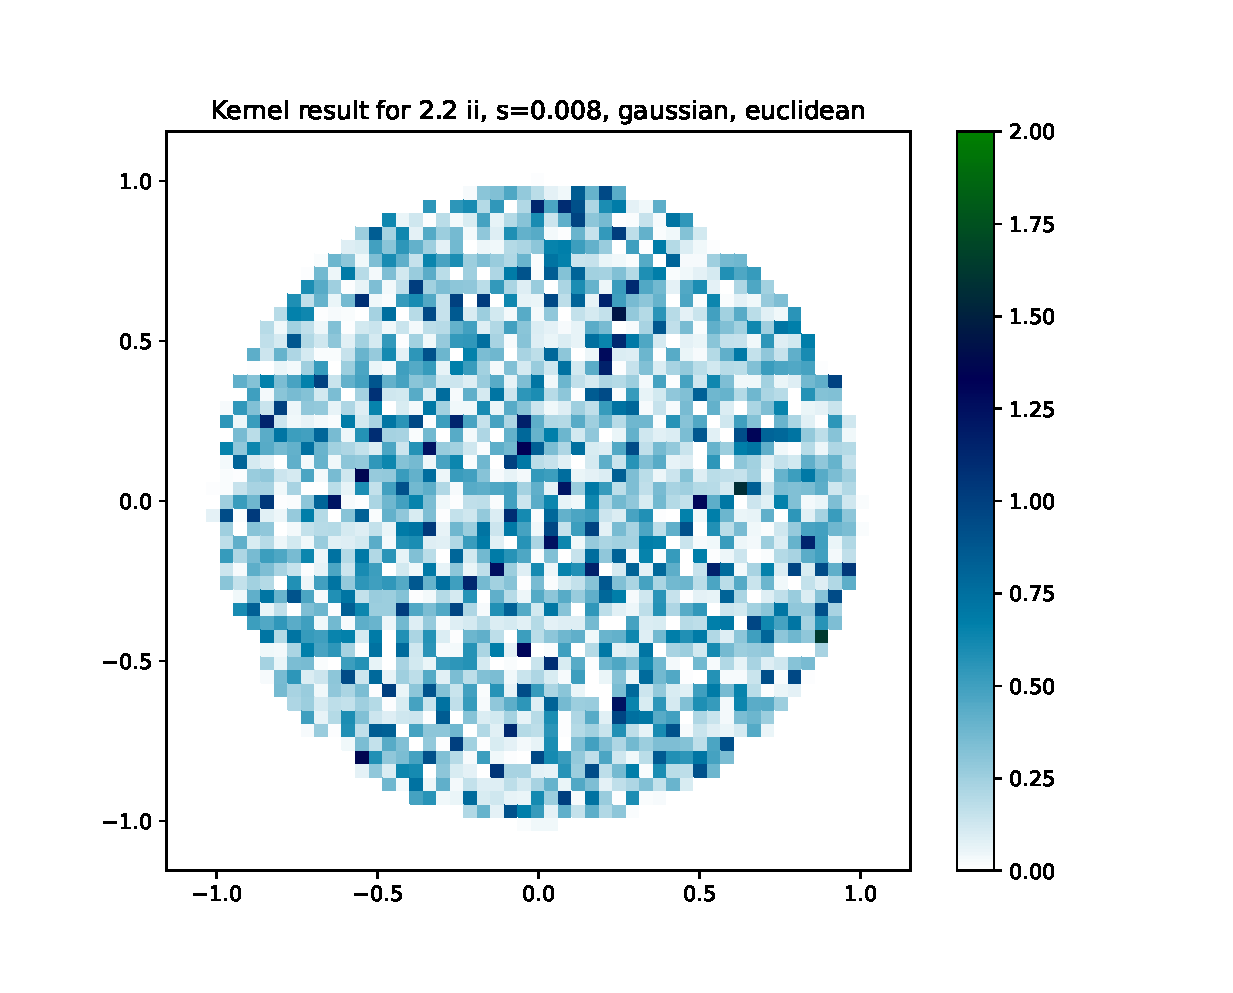
\includegraphics[height=8cm]{comparisons//Kernel_result_2-2ii_s_0-008_gaussian_euclidean.eps}  \\
\hspace*{-1.5cm}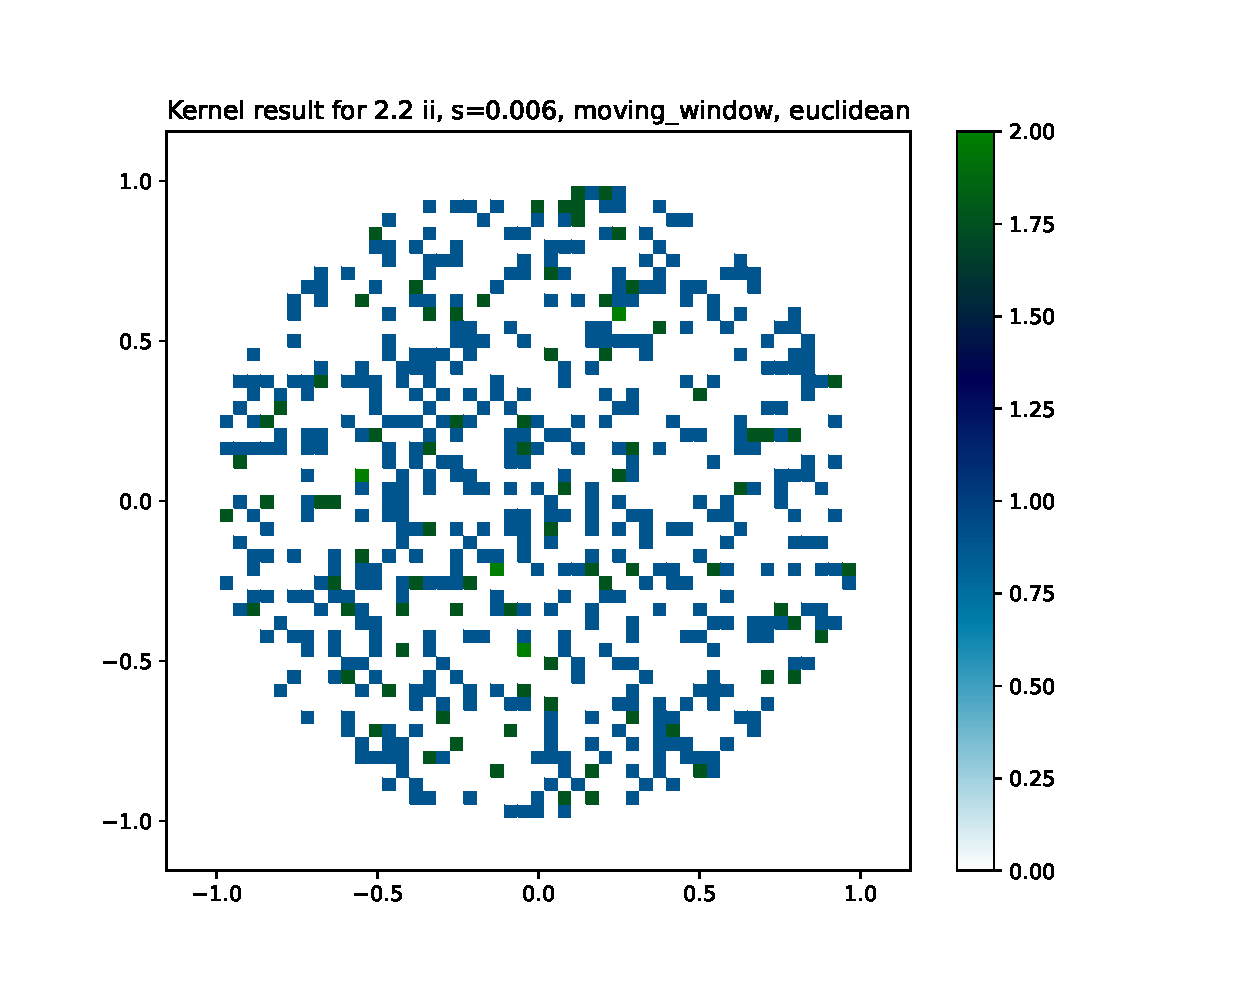
\includegraphics[height=8cm]{comparisons//Kernel_result_2-2ii_s_0-006_moving_window_euclidean.eps} \hspace*{-1.5cm}
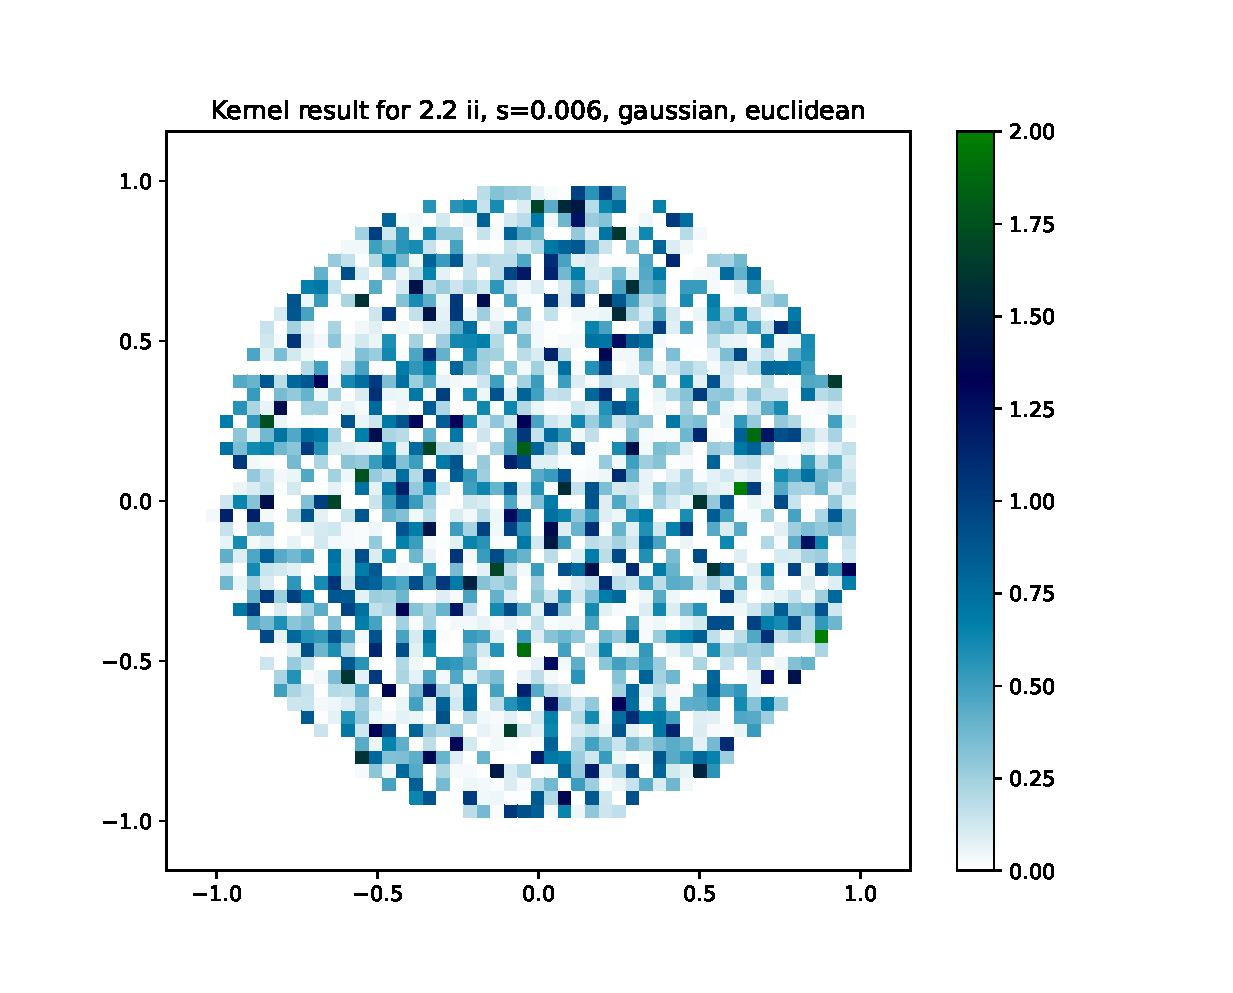
\includegraphics[height=8cm]{comparisons//Kernel_result_2-2ii_s_0-006_gaussian_euclidean.eps}  \\
Intuitively, the Gaussian kernel seems to outperform the Moving Window Kernel, since the plots of Gaussian kernel are "blurer". \vspace*{0.8em}\\
Let us denote $h$ as the density of the unit Euclidean ball in $\mathbb{R}^2$. \\
To take a closer look at the comparison between Moving Window and Gaussian kernels as well as between $||\cdot ||_2$ and $||\cdot ||_{\infty}$, we also implement a function that very roughly calculates $||h-h_{K,D,s}||_{\mathcal{L}_1}$ by treating the $h_{K,D,s}$ values of all points in a grid as the same. The results are as follows: \vspace*{-0.6cm}\\

\begin{multicols}{2}


\begin{center}

Rough $L_1$-Norm Comparison  between $||\cdot ||_2$ and  $||\cdot ||_{\infty}$ for Moving Window kernel \vspace*{1em} \\
\begin{tabular}{ccc}

\hline  

$s$  &$||\cdot||_2$              &$||\cdot||_{\infty}$   \\
\hline  

0.006      &2.26396      &2.65265\\
0.008	    &2.54605   &2.07668 \\
0.01	    &1.68825   &2.2102 \\
0.02	    &4.53346   &5.29291 \\
0.03	    &7.55802   &8.46946 \\
0.04	    &9.37843   &11.04753 \\
0.06	    &14.4997   &16.35089 \\
0.08	    &19.76346   &22.89573 \\
0.1	    &24.28602   &27.41789 \\

\hline 
\end{tabular}
\end{center}


\begin{center}
Rough $L_1$-Norm Comparison  between Moving Window $\&$ Gaussian under $||\cdot||_2$ \vspace*{1em} \\
\begin{tabular}{ccc}

\hline  

$s$  &Moving Window              &Gaussian   \\
\hline  

0.006      &2.26396   &2.00969\\
0.008	    &2.54605   &2.0962 \\
0.01	    &1.68825   &2.53684 \\
0.02	    &4.53346   &6.16157 \\
0.03	    &7.55802   &9.56693 \\
0.04	    &9.37843   &12.88424 \\
0.06	    &14.4997   &19.32132 \\
0.08	    &19.76346   &25.22606 \\
0.1	    &24.28602   &30.50908 \\

\hline 
\end{tabular}

\end{center}

\end{multicols}

\noindent From the above tables, we can see that with smaller $s$, the approximative $||h-h_{K,D,s}||_{\mathcal{L}_1}$ value firstly decreases, but for $s<0.01$, it seems to be larger again. Moreover, $||\cdot||_2$ delivers a slightly smaller approximative value than $||\cdot||_{\infty}$. These two observations align with our previous unrigorous hypothesis. However, the approximative $||h-h_{K,D,s}||_{\mathcal{L}_1}$ value delivered from Moving Window kernel is slighty better than that from Gaussian, which is contrary to our naive imagination.\\
We conclude that further  mathematical knowledge is of urgency for further analysis... 

\section*{Exercise 2.14} \vspace*{-1em}
Let $(X,\mathcal{A},\mu)$ be a finite measure space and $\mathbf{P}$ be a $\mu$-absolutely continuous probability measure with \textit{known} $\mu$-density $h$. For a given \textit{known} density estimate $\hat{h}:X \rightarrow [0,\infty)$ find a computationally efficient method to approximately compute $||h-\hat{h}||_{\mathcal{L}_1(\mu)}$. Implement this method and apply it to the experiments conducted in Exercise 2.3. Compare your findings with those of Exercise 2.11. \vspace*{0.5em}\\
\textit{Assumptions:}\\
For a $d\in \mathbb{N}$, $X=\mathbb{R}^d, \mathcal{A} = \mathcal{B}^d, \mu = \lambda ^d $.\\
$h, \hat{h}$ are "\textit{known}"\,in the sense that for $\forall x\in \mathbb{R}^d:$ we explicitly know the value of $h(x)$ and $\hat{h}(x)$.  \vspace*{0.5em}\\
$h, \hat{h}$ are bounded functions. \\
\textit{Solution:}\\
Under to our assumptions, we can find a $\mu$-adapted cubic partition $\mathfrak{A} = (A_j)_{j\in \mathbb{N}}$ of width $s$ for $X$.  \\
For an arbitrary cell $A_j\in \mathfrak{A}$,  notice that $\overline{A_j} \in \mathcal{A} \ \land \  \mu(\overline{A_j}\backslash A_j) = 0 $. \vspace*{0.5em}  \\
$\Rightarrow \ \displaystyle{ \int_{A_j}   h\, \text{d} \mu =  \int_{\overline{A_j}} h \,  \text{d} \mu } \ \land \  \displaystyle{ \int_{A_j}   \hat{h}\, \text{d} \mu =  \int_{\overline{A_j}} \hat{h} \,  \text{d} \mu }  $ . \vspace*{0.5em}   \\
Denote $h_j := h_{\overline{A_j}}$ and $\hat{h}_j := \hat{h}_{\overline{A_j}}$.\\ 
Obviously $h_j$, $\hat{h}_j$ are real functions defined on a compact set. \vspace*{0.5em} \\
$\Rightarrow \ $ $h_j$, $\hat{h}_j$ are Riemann-integrable  $\land \  \displaystyle{ \int_{A_j} h\, \text{d} \mu =  \int_{\overline{A_j}} h_j (x) \,\text{d}x   } \ \land \ \displaystyle{ \int_{A_j} \hat{h} \, \text{d} \mu =  \int_{\overline{A_j}} \hat{h}_j (x) \,\text{d}x   }  $. \vspace*{0.5em} \\
Combining the above considerations together, we obtain: \vspace*{0.5em}  \\
$|| h-\hat{h} ||_{\mathcal{L}_1 (\mu)} = \displaystyle{ \int_X |h-\hat{h}|\,\text{d}\mu = \int_{ \bigsqcup_{j\in \mathbb{N}} A_j  } |h-\hat{h}|\,\text{d}\mu = \sum_{j\in \mathbb{N}} \int_{ A_j  } |h-\hat{h}|\,\text{d}\mu =  \sum_{j\in \mathbb{N}} \int_{ \overline{A_j}  } |h(x)-\hat{h}(x)|\,\text{d}x   }$.\vspace*{0.5em}  \\
Our idea is to approximate the the desired quantity with the Riemannian sum for very small $s$. This means that:  \vspace*{0.5em}  \\
For an $x_j \in A_j: \displaystyle{ \int_{ \overline{A_j}  } |h(x)-\hat{h}(x)|\,\text{d}x = \int_{ \overline{A_j}  } |h(x_j)-\hat{h}(x_j)|\,\text{d}x \approx s^2 |h(x_j)-\hat{h}(x_j)|    }$.\vspace*{0.5em}  \\
Therefore, for very small $s$ and the respective $\mathfrak{A}=(A_j)_{j\in \mathbb{N}}$, we can choose a set of grid points $(x_j)_{j\in \mathbb{N}}$ with $x_j \in A_j$ and obtain: \vspace*{0.5em}  \\ 
 $|| h-\hat{h} ||_{\mathcal{L}_1 (\mu)} = \displaystyle{ \sum_{j\in \mathbb{N}} \int_{ \overline{A_j}  } |h(x)-\hat{h}(x)|\,\text{d}x  =  \sum_{j\in \mathbb{N}} s^2 |h(x_j)-\hat{h}(x_j)|   } $. \vspace*{0.8em}  \\ 
\textit{Implementation Strategy:}\\
On a practical level, it is impossible for a computer to deal with an infinite set of grid points, but since $\hat{h}$ is obtained from a (hopefully large enough) data set, we can consider only the area that bounds the data set to be a set that covers the support of $h$, namely we consider $[a,b]\subseteq X $ with $ D\subseteq [a,b]$ to have the property $\text{supp}h \subseteq [a,b]$. \\
For a very small $s$, we then generate a set of equidistant grid points in $[a,b]$ and conduct the calculations introduced above. \\
For a histogram $h_{D,s'}$, we also need to garantee that the new grids generated through $[a,b]\supseteq D$ and $s$ are a refinement of the partition used to generate $h_{D,s'}$. \\
\newpage 
Due to time limit, we have only tested our method on the distribution of the unit Euclidean ball. \\
The result is as follows: 


\begin{center}
$||h-h_{D,s}||_{\mathcal{L}_1(\mu)}$ for the Distribution of the Unit Euclidean Ball with $|D|=30,000$ \vspace*{1em} \\
\begin{tabular}{ccc}

\hline  

$s$  &$||h-h_{D,0.01}||_{\mathcal{L}_1(\mu)}$   \\
\hline  

1    &0.651643219517124\\
0.5    &0.25375586178738563\\
0.25    &0.0880281605675654\\
0.1    &0.0474178390241438\\
0.075    &0.03204401378043235\\
0.05    &0.026396712601441177\\
0.025    &0.01430751148369362\\
0.01    &0.0055766195804626585\\
0.0075    &0.0041858449609556495\\
0.005    &0.0028030985260043273\\
0.0025    &0.0014052464469453995\\
0.001    &0.0005629859029245468\\
0.00075    &0.00042227322994948125\\
0.0005    &0.0002816408388199983\\
0.00025    &0.0001408573912494324\\
0.0001    &5.635182974124233e-05\\
7.5e-05    &4.2264210333481576e-05\\
5e-05    &2.8177393744205783e-05\\
2.5e-05    &1.4089066590475308e-05\\
1e-05    &5.635715368618041e-06\\


\hline 
\end{tabular}

\end{center}

\noindent We can see that as $s$ decreases, the value $||h-h_{D,0.01}||_{\mathcal{L}_1(\mu)}$ also decreases. \\
However, the value $||h-h_{D,0.01}||_{\mathcal{L}_1(\mu)}$ seems to keep approaching 0 and this seems to be strange...









\end{document}